\documentclass[main.tex]{subfiles}
\begin{document}


\chapter{Search for $\beta\beta$ decay of $^{\text{116}}$Cd into the excited states of $^{\text{116}}$Sn}



%\begin{flushright}


%\textit{You see, mon ami, the voices of the little gray cells have begun to sing to Poirot.}\\
%Agatha Christie, \textit{Appointment with Death}.
%\end{flushright}



%\bigskip


\NI The investigation of the $\beta\beta$ decays of $^{\text{116}}$Cd via the excited states of $^{\text{116}}$Sn is described in this section. These decays are expected to be even rarer than the decay to the ground state but their very clear signature topology, simultaneous emission of two electrons accompanied by one or more photons, allow their searches with a high background suppression.


\bigskip


\NI The two main excited states of $^{\text{116}}$Sn are introduced in Section~\ref{sec:ESCd}. The analysis technique used to perform the search is described in Section~\ref{sec:AnalysisTechnique}. The modelisation of the background and the measurement of its different contributions are presented in Section~\ref{sec:BKGexcitedStates}. The preselection criteria of the events for these decay channels are described in Section~\ref{sec:Preselection}. The optimisation of the cuts using a multivariate approach is presented in Section~\ref{sec:CutOptimisation}. The evaluation of the sources of systematic uncertainties is discussed in Section~\ref{sec:SourceOfSystematics}. The results of these searches are presented in Section~\ref{sec:Result2PLUS} and Section~\ref{sec:Result0PLUS} for the two main excited states respectively in both 2$\nu$ and 0$\nu$ decay modes. Finally the results are summarised in Section~\ref{sec:SummaryAnalysis}.


\section{Excited states of \texorpdfstring{$^{\text{116}}$}~Sn}
\label{sec:ESCd}


\NI The search for the 2$\nu\beta\beta$ and 0$\nu\beta\beta$ decays to the ground state have been investigated with the full statistic of NEMO-3~\cite{Arnold2016bed}. In theory, the $\beta \beta$ decays can also occur through the excited states of the daughter nucleus. Due to smaller space phases these decays to the excited states are even rarer than the decay to the fundamental state but some of them have already been observed for $^{\text{100}}$Mo and $^{\text{150}}$Nd nuclei~\cite{Barabash2010ie}. Concerning the \Cd, the $\beta \beta$ decays via the excited have never been found. The results of this analysis will lead to the first values or limits put on these processes with the NEMO-3 data.


\bigskip


\NI The searches for $\beta \beta$ decays through the excited states is mainly motivated by a better understanding of the nuclear structures. The measurement of the decay rate could brings informations on nuclear matrix elements, which are sensitive to nuclear-spin isospin correlations, and provide additional handle for NME calculations. The decays via the excited states are also interesting to investigate the 0$\nu\beta\beta$ mechanism by giving us alternative channels to study an hypothtical 0$\nu\beta\beta$ signal. Finally, they also offer us the possibility to distinguish between the various 0$\nu\beta\beta$ mechanisms since the branching ratios of 0$\nu\beta\beta$ decay between the excited states and the ground state could differ according the model~\cite{TheoryOfNeutrinolessDBD}.


\bigskip


\NI The simplified schema of the \Cd~decay to \Sn~is shown in Figure \ref{SchemaExcitedState}. Only the 2 first excited states are considered at 1294 keV (2$^+$) and at 1757 keV (0$^+$). These two excited states will be studied in case of 2$\nu\beta\beta$ and 0$\nu\beta\beta$. The label and the description of each case are given below :



\begin{itemize}
\item \textbf{(0$^+$) 2$\nu$} : The signature of this decay is the simultaneous emission of 2~electrons and 2~photons. The Q$_{\beta \beta}$ of the electron energy spectrum is 1048 keV. The photon energy spectrum is very characteristic with two peaks at 463 keV and 1294 keV.

\item \textbf{(0$^+$) 0$\nu$} : The signature of this decay is the simultaneous emission of 2~electrons and 2~photons. As no neutrino is emitted, the electron energy sum spectrum is peaked at 1048 keV. The photon energy spectrum is the same than in (0$^+$) 2$\nu$.

\item \textbf{(2$^+$) 2$\nu$} : The signature of this decay is the simultaneous emission of 2~electrons and 1~photon. The Q$_{\beta \beta}$ of the electron energy spectrum is 1511 keV. The gamma energy spectrum is characterized by a peak at 1294 keV.

\item \textbf{(2$^+$) 0$\nu$} : The signature of this decay is the simultaneous emission of 2~electrons and 1~photon. The electron energy sum spectrum is caracterized by a peak at 1511 keV. The photon energy spectrum is the same than in (2$^+$) 2$\nu$.
\end{itemize}



\begin{figure} [h!]
\begin{center}
\includegraphics[scale=0.60]{pictures/Chap6/SchemaCdExcitedState.pdf}
\end{center}
\caption{Schema of the two main excited of $^{\text{116}}$Sn. The excited state 0$^+$ (1757 keV) corresponds to the emission of two electrons with a Q$_{\beta\beta}$~=~1048~keV and two photons at~1294~keV and 463~keV. The excited state 2$^+$~(1294~keV) corresponds to the emission of two electrons with a Q$_{\beta\beta}$~=~1511~keV and one photon at~1294~keV. In case of 2$\nu\beta\beta$ these decays are accompagnied by two neutrinos.}
\label{SchemaExcitedState}
\end{figure}



\NI Theoretically, the decay probability to the excited states is proportionnal to (Q$_{\beta\beta}$~$-$~E$^*$)$^{\text{11}}$ in 2$\nu\beta\beta$ decay and to (Q$_{\beta\beta}$ $-$ E$^*$)$^{\text{5}}$ in 0$\nu\beta\beta$ decay, where Q$_{\beta\beta}$ is the total available energy and E$^*$ the energy of the excited state. It can be deduced that the decay to the excited state~2$^+$ is more likely than the decay via~0$^+$. Furthermore, as the detection efficiency of the electrons increases with the their energy, the decays via the excited state 2$^+$ seems easier to detect. One the other hand, the presence of two electrons and one photon inside the detector is more reproducible by the background than the presence of two electrons and two photons. In any case, the detection efficency of the two electrons and one or more photons will be very low. It explains why the search for decays via the excited states is very challenging with the NEMO-3 detector.


\bigskip


\NI Historically, the first observation of the \Cd~ 2$\nu\beta\beta$ decay was reported in 1995 by three independent experiments : NEMO-2~\cite{Barabash2010ie}, Elegant-V~\cite{ElegantV-1} and at the Solotvina Underground laboratory\cite{Aurora}. NEMO-2 was installed at LSM and took data during ten months with a enriched cadmium source surrounded by tracking chamber and plastic scintillator calorimeter. The half-life of 2$\nu\beta\beta$ was measured to be T$_{\text{1}/\text{2}}^{\text{2}\nu}$~=~(3.75 $\pm$ 0.35 (stat) $\pm$ 0.21~(syst)~)~$\times$~10$^{\text{19}}$~y. Limit at 90\% C.L on the \Cd~half-lives of T$_{\text{1}/\text{2}}^{\text{0}\nu}$~>~5.0~$\times$~10$^{\text{21}}$ y for 0$\nu\beta\beta$ decay were obtained with an exposure of 0.11~kg$\times$y. In the same time, ELEGANT-V reported the results of the double beta decay using natural and enriched cadmium foils sandwiched between drift chambers and plastic scintillators. Sodium iodide scintillators was used to enhance background rejection. The half-life have been measured to be T$_{\text{1}/\text{2}}^{\text{2}\nu}$~=~2.6 $^{+\text{0.9}}_{-\text{0.5}}$~$\times$~10$^{\text{19}}$~y with an exposure of 0.02~kg$\times$y. A lower limit on the 0$\nu\beta\beta$ was set to T$_{\text{1}/\text{2}}^{\text{0}\nu}$ > 2.9~$\times$~10$^{\text{21}}$~y. These measurements are compatible with the results obtained with cadmium tungstate crystal scintillators at the Solotvina Underground Laboratory.  The half-life of 2$\nu\beta\beta$ was measured to be T$_{\text{1}/\text{2}}^{\text{2}\nu}$~=~2.7$^{+\text{0.5}}_{-\text{0.4}}$~$\times$~10$^{\text{19}}$~y. The lower limit on the half-life was set to T$_{\text{1}/\text{2}}^{\text{0}\nu}$~>~2.9~$\times$~10$^{\text{22}}$~y at 90\%C.L. 


\bigskip


\NI More recently the study of the \Cd~decay has continued mainly using CdWO$_{\text{4}}$ scintillator crystals. The Solotvina experiment reported the results obtained with 330 g of crystals for a total exposure  of 0.4~kg$\times$y~\cite{Solotvina}. The 2$\nu\beta\beta$ half-life corresponding to T$_{\text{1}/\text{2}}^{\text{2}\nu}$~=~[2.9 $\pm$ 0.06 (stat.) $^{+\text{0.4}}_{-\text{0.3}}$ (syst.)]~$\times$~10$^{\text{19}}$~y. Installed at the Gran Sasso Underground Laboratory, the Aurora experiment investigate double beta decay of \Cd~ with 1.162~kg of crystal scintillators enriched to 82~\%~\cite{Aurora}. The half-life of 2$\nu\beta\beta$ was measured to be T$_{\text{1}/\text{2}}^{\text{2}\nu}$~=~[2.62 $\pm$ 0.14]~$\times$~10$^{\text{19}}$~y for the ground state. The lower limit on the half-life was set to T$_{\text{1}/\text{2}}^{\text{0}\nu}$~>~1.7~$\times$~10$^{\text{23}}$~y at 90\%~C.L. Aurora has also puts new limits concerning the decay of \Cd~via the excited state of \Sn. The main results obtained for 2$\nu\beta\beta$ and 0$\nu\beta\beta$ decays to the ground and the excited states are gathered in Table~\ref{TableSummaryResultsFS}.



\begin{table}[h!]
\begin{center}
\begin{tabular}{c|c|c|c}
\toprule
Experiment & Decays & T$_{\text{1}/\text{2}}$ half-life or limit [y] at 90 \% C.L & ref\\[0.1cm]
\hline

\multirow{2}{*}{NEMO-2} & 2$\nu$ (g.s) & [3.75 $\pm$ 0.35 (stat.) $\pm$ 0.21 (syst.)]~$\times~$10$^{\text{19}}$&  \multirow{2}{*}{\cite{NEMO2:Cd116}}\\[0.1cm]
                        & 0$\nu$ (g.s) & $>$ 5~$\times$~10$^{\text{22}}$ &\\[0.1cm]
                                               
\hline   
\multirow{2}{*}{NEMO-3}  & 2$\nu$ (g.s) & [2.74 $\pm$ 0.04 (stat.) $\pm$ 0.18 (syst.)]~$\times$~10$^{\text{19}}$& \multirow{2}{*}{\cite{Arnold2016bed}}\\[0.1cm]
                        & 0$\nu$ (g.s) & $>$ 1.0~$\times$~10$^{\text{23}}$ &\\[0.1cm]
                    
\hline                        

\multirow{2}{*}{ELEGANT-V}  & 2$\nu$ (g.s) & [2.6 $^{+\text{0.9}}_{-\text{0.5}}$]~$\times$~ 10$^{\text{19}}$& \multirow{2}{*}{\cite{ElegantV-1}}\\[0.1cm]
                           & 0$\nu$ (g.s) & $>$ 2.9~$\times$~10$^{\text{22}}$ &\\[0.1cm]
                        
                        
\hline

%\multirow{2}{*}{CdWO$_{\text{4}}$} & 2$\nu$ (g.s) & [2.7 $^{+\text{0.5}}_{-\text{0.4}}$~(stat.)~$^{+\text{0.9}}_{-\text{0.6}}$~(syst.)]~$\times$~10$^{\text{19}}$& a\\[0.1cm]
%                           & 0$\nu$ (g.s) & $>$ 2.9~$\times$~10$^{\text{22}}$& \\[0.1cm]

%\midrule
                           
                           
\multirow{2}{*}{Solotvina} & 2$\nu$ (g.s) & [2.9 $\pm$ 0.06 (stat.)~$^{+\text{0.4}}_{-\text{0.3}}$ (syst.)]~$\times$~10$^{\text{19}}$& \multirow{2}{*}{\cite{Solotvina}}\\[0.1cm]
                           & 0$\nu$ (g.s) & $>$ 1.9~$\times$~10$^{\text{23}}$ &\\[0.1cm]
                           

\hline

\multirow{6}{*}{Aurora} & 2$\nu$ (g.s) & [2.62~$\pm$ 0.06~(stat.)~$\pm$~0.14~(syst.)]~$\times$~10$^{\text{19}}$& \multirow{6}{*}{\cite{Aurora}}\\[0.1cm]
                        & 2$\nu$ (0$^+$) & $>$ 9.0~$\times$~10$^{\text{20}}$&\\[0.1cm]
                        & 2$\nu$ (2$^+$) & $>$ 1.0~$\times$~10$^{\text{21}}$&\\[0.1cm]
                        & 0$\nu$ (g.s)   & $>$ 1.9~$\times$~10$^{\text{23}}$&\\[0.1cm]
                        & 0$\nu$ (0$^+$) & $>$ 6.2~$\times$~10$^{\text{22}}$&\\[0.1cm]
                        & 0$\nu$ (2$^+$) & $>$ 6.3~$\times$~10$^{\text{22}}$&\\[0.1cm]
\bottomrule
\end{tabular}
\caption{Summary of results for the search for $\beta \beta 2\nu$ and $\beta \beta 0\nu$ decays to the fundamental and excited states.}
\label{TableSummaryResultsFS}
\end{center}
\end{table}


\FloatBarrier

\clearpage

\section{Analysis technique}\label{sec:AnalysisTechnique}


\NI The NEMO-3 analysis technique consists of a comparison of the experimental data obtained by the detector to the Monte-Carlo simulations of physics processes such as double beta decay. The simulated data are then propagated throught the NEMO-3 detector by GEANT-3. Section~\ref{sec:MCsimu} presents the event generation and their propagation in the detector. Both simulated and real data are then reconstructed with a dedicated software package developed by the collaboration. Section~\ref{sec:RecoNEMOR} introduces the event reconstruction which provides the informations necessary for building the objects used in particle identification. The particle identification, presented in Section~\ref{sec:PIDanalysis}, and the timing informations, shown in Section~\ref{sec:TOFanalysis}, are then used to identify different independant analysis channels. Section~\ref{sec:StatAnalysisTools} describes the statistical tools used to measure the background, to set limits or to optimise the selection. Finally, Section~\ref{sec:HalfLifeAnalysis} presents the method used to translate decay rates measured with NEMO-3 data into half-lives.


\subsection{MC simulation}\label{sec:MCsimu}


\NI The Monte Carlo simulations for NEMO-3 are generated using the GENBB event generator~\cite{GENBB}. This program, which is a particular implementation of DECAY0 used by NEMO-3, provides the initial state of the particles with accurate kinematics, timing and branching ratio. GENBB generates all the necessary informations on 2$\nu\beta\beta$ and 0$\nu\beta\beta$ decay modes and also on the different decays used for the background isotopes.


\bigskip


\NI The transport of the particles generated by GENBB through NEMO-3 is simulated by GEANT-3.21 \cite{GEANT3} which uses a full description of the detector. GEANT-3.21 simulates the interactions of the particles in all of the simulated detector components. The simulated data are then digitized in exactly the same format as raw data in a way to use the same reconstruction process.   


\subsection{Event reconstruction}\label{sec:RecoNEMOR}


\NI The real and simulated data are reconstructed and calibrated in a same way thanks to a dedicated software package called NEMOR. This program uses the digitized informations to produce the physical objects used in the NEMO-3 data analysis. 


\bigskip


\NI In order to take into account the different data taking conditions, and ensure that MC events can be directly compared to the real data, all the MC sample events are distributed into several run periods according to the length of the real data runs.  This can be performed thanks to the existence of a database containing all the informations relative to the real detector running conditions such as the life time of each run. The database also contains the status of each PMTs and each Geiger cells during the lifetime of the experiment. All these informations such as the dead channel or the real-time calibration coefficients can be used during the reconstruction of the simulated data in order to be as close as possible to the data acquisition conditions.  


\subsubsection{Track reconstruction}


\NI The reconstruction of the particle track inside the tracker is performed in NEMOR software. During the passage of a charged particles in the tracker, the wires close to its passage are triggered and constitute the building blocks for the tracking pattern recognition algorithm. According the transverse and longitudinal hit positions and the timing informations, the hits are clustered together using a cellular automated tracking algorithm. This algorithm searches for successive hits in the neighbouring layers and connects them with simple line segments. This proccess continues until there are no more consecutive hits. When all the segments are been added to the cluster, they are removed from the search and a new one startes until there are not segments available to build a track. After the identification of all the tracks in the events, three helical fits are performed for each track. The first fit, which is global, uses all the hits contains in the track cluster. This fit provides the measurement of the track length. The two others fits are performed by using only the hits closest to the source foil and closest to the calorimeter wall to precisely measure the vertex position on the source foil and the impact point on the calorimeter block.


\subsection{Particle identification}\label{sec:PIDanalysis}


\NI By using the different reconstructed informations provided by the tracker and calorimeter, NEMO-3 give us the ability to distinguish between different types of particles. The identifiable particles in NEMO-3 data are electrons, positrons, photons and alpha particles.


\subsubsection{Electron identification}


\NI Electrons and positrons are identified as curved tracks inside the tracker. The track must intersect the source foil and be associated to a single calorimeter hit. Thanks to the magnetic field, the distinction between electrons and positrons can be performed by looking at their opposite curvature. Figure~\ref{DoubleBetaEventDisplay} shows an event where two electrons have been identified in the NEMO-3 data. In order to properly reconstructed the full energy of the electrons, the neighbouring optical modules, side and diagonally, must not been fired. If neighbouring optical modules have hit, this could be explained by a scaterring off of the first optical module to a close one. In this kind of event, the trajectory of the particle is not well reconstructed by the tracking algorithm. These events are associated with a large systematic uncertainties or can be removed from the analysis.


\begin{figure}[h!]
\centering
\includegraphics[scale=0.35]{pictures/Chap6/betabetaEvent.png}
\label{DoubleBetaEventDisplay}
\caption{Top view of the NEMO-3 detector where two electron candidates have been identified in the NEMO-3 data. The red and blue lines are the reconstructed tracks, the small circles corresponds to to the Geiger hits. Their sizes depend on the distance between the particle track and the anode wire. The blue boxes are the inner and outer calorimeter walls. The location of the calorimeter hits are colored in yellow. The magenta boxes represents the petal scintillators.}
\end{figure}

\FloatBarrier

\subsubsection{Photon identification}


\NI Contrary to the electrons and positrons, the photons are not charged, so do not leave a track in the tracker volume. Moreover, as the detection efficiency for a photon of 0.5~MeV is 60~\%, nothing guarantee that the photon is fully contained in a single or isolated calorimeter hits. Photons are identified as an energy deposit in one or several optical modules without an associated track. During the photon identification, the neighbouring calorimeter hits are clustered and attributed to a single photon. The energy of the photon being equal to the sum of the individual hits energies. Examples of neighbouring calorimeters hits which could be gather together are shown in Figure~\ref{GammaClusterSchema}. Futhermore, no Geiger cell that are unassociated to tracks may be found within 15~cm radially of calorimeter hits in order to limit the mis-identification from $\alpha$ decay (next section) or scattered electrons as photons.


\begin{figure}[h!]
\centering
\includegraphics[scale=0.35]{pictures/Chap6/GammaCluster.png}
\label{GammaClusterSchema}
\caption{Schematic front view of the main wall. The grid represents scintillator blocks. The red squares correspond to optical modules with energy deposits without associated tracks. They could be clustered to form a photon.}
\end{figure}

\FloatBarrier

\subsubsection{Alpha identification}


\NI As it was already described in Chapter~5, due to their high ionizing power and to the high mass, the alpha particles are identified as short straight lines. The alpha particles from radioactive decay are not expected to be higher than 40~cm.


\bigskip


\NI The identification of the alpha particle is important to detect the Bi-Po cascades in which an alpha decay with a half-life of 164~$\mu$s occurs. The BiPo cascade is then identify as the emission of a prompt electron followed by a delayed alpha coming from the same location as shown in Figure~\ref{AlphaNEMO3}.  


\begin{figure}[h!]
\centering
\includegraphics[scale=0.4]{pictures/Chap6/alphaIdentification.png}
\label{AlphaNEMO3}
\caption{Top view of the NEMO-3 detector where a candidate BiPo event have been identifed. The red track corresponds to the prompt electron while the black squares represents the delayed Geiger hits of the alpha track.}
\end{figure}


\FloatBarrier

\subsection{Time of flight informations}\label{sec:TOFanalysis}


\NI The $\beta\beta$ signal is characterized by the emission of two electrons coming from the source foil in coincidence in time. To measure a signal or a background coming from the source it is necessary to reduce as much as possible the contribution of the events from an external origin. To distinguish the origin of the events, internal or external to the source foil, the time of flight informations provided by the calorimeter is used. Two different hypotheses, internal and external are introduced which quantify the probability that a event has its origin inside or outside the source foil. These two probabilities are build out of $\chi^\text{2}$ distributions using the measured time of particle hits in the calorimeter and the hypothetical time of flight calculated from the estimated speed and the trajectory of the particle between its vertex to the calorimeter. The $\chi^\text{2}$ calculations also take into account the uncertainties on the measured and hypothetical times. Next sections present the calculation of the internal and external hypotheses. These hypotheses are calculated between two particles. One of the particle must be an electron with a reconstructed track and vertex.  The other particle can be a second electron or a photon. According the kind of particle the uncertaities are not computed in the same way as explained at the end of the section.


\subsubsection{Internal probability}\label{sec:Pint}


\NI The internal hypothesis $\chi_{\text{int}}$ assumes that the two detected particles come from the same decay occuring at a time t$_\text{0}$ inside the source foil :


\begin{equation}
\text{t}_\text{1}^{\text{mes}} - \text{t}_\text{1}^{\text{tof}} = \text{t}_\text{0} = \text{t}_\text{2}^{\text{mes}} - \text{t}_\text{2}^{\text{mes}}  
\end{equation}


\NI where $\text{t}_\text{1}^{\text{mes}}$ and $\text{t}_\text{2}^{\text{mes}}$ are the measured time of particle hits 1 and 2 in the calorimeter, and $\text{t}_\text{1}^{\text{tof}}$ and $\text{t}_\text{2}^{\text{tof}}$ are the hypothetical time of arrival of the particle 1 and 2. By taking account the uncertainties on each of these parameters, the internal pull is defined as :


\begin{equation}
\chi_{\text{int}} = \frac{(\text{t}_\text{1}^{\text{mes}} - \text{t}_\text{1}^{\text{tof}}) - (\text{t}_\text{2}^{\text{mes}} - \text{t}_\text{2}^{\text{mes}} ) }{\sqrt{ \sigma^{\text{2}}_{\text{t}_\text{1}^{\text{mes}}} + \sigma^{\text{2}}_{\text{t}_\text{1}^{\text{tof}}} + \sigma^{\text{2}}_{\text{t}_\text{2}^{\text{mes}}} + \sigma^{\text{2}}_{\text{t}_\text{2}^{\text{tof}}}  }}
\end{equation}


\NI Then, the internal probability P$_{\text{int}}$ is defined from $\chi_{\text{int}}$ as : 


\begin{equation}\label{eq:probaDef}
\text{P}_{\text{int}} = \text{1} - \frac{\text{2}}{\pi} \int_\text{0}^{\chi^\text{2}_{\text{int}}} \text{e}^{\text{x}^\text{2}} \text{dx}
\end{equation}


\NI with x defined as :

\begin{equation}
\text{x} = \frac{\text{1}}{\text{1}+\sqrt{\text{2}\chi^\text{2}_{\text{int}}}}
\end{equation}


\NI The internal probability for an internal and an external 2-e event is shown in Figure~\ref{PintforIntandExt}. For an internal event the distribution is expected to be constant while is expected to be peaked for an external event.


\begin{figure}[h!]
\centering
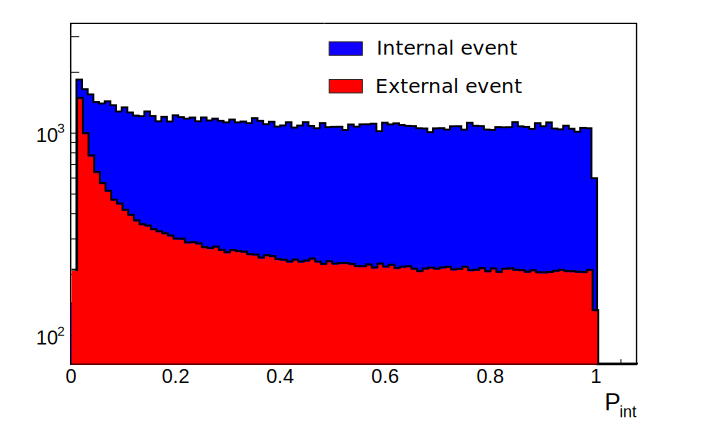
\includegraphics[scale=0.55]{pictures/Chap6/Pint_explication.pdf}
\label{PintforIntandExt}
\caption{Internal probability distribution for an internal 2-e event in blue and for an external event in red.}
\end{figure}



\FloatBarrier


\subsubsection{External probability}\label{sec:Pext}


\NI The external hypothesis is built as the internal hypothesis exept that the vertex of the decay is assumed to be outside the source foil. Figure~\ref{ExternalEventDisplay} shows two typical external events in which a 2-e event is induced by a external photon. According which particle generates the other two different external hypotheses are constructed : 


\begin{equation}
(\text{1} \rightarrow \text{2})~~~~~ \text{t}_\text{1}^{\text{mes}} = \text{t}_\text{0} = \text{t}_\text{2}^{\text{mes}} - \text{t}_\text{2}^{\text{tof}} - \text{t}_\text{1}^{\text{tof}}
\end{equation}

\begin{equation}
(\text{2} \rightarrow \text{1})~~~~~ \text{t}_\text{2}^{\text{mes}} = \text{t}_\text{0} = \text{t}_\text{1}^{\text{mes}} - \text{t}_\text{1}^{\text{tof}} - \text{t}_\text{2}^{\text{tof}}
\end{equation}


\NI By considering only the first expression (1 $\rightarrow$ 2), the associated $\chi^\text{2}_{\text{ext}}$ is defined as : 

\begin{equation}
(\text{1} \rightarrow \text{2})~~~~~ \chi^\text{2}_{\text{ext}} = \frac{ (\text{t}_\text{2}^{\text{mes}} - \text{t}_\text{2}^{\text{tof}} - \text{t}_\text{1}^{\text{tof}} - \text{t}_\text{1}^{\text{mes}} )^\text{2} }{  \sigma^{\text{2}}_{\text{t}_\text{1}^{\text{mes}}} + \sigma^{\text{2}}_{\text{t}_\text{1}^{\text{tof}}} + \sigma^{\text{2}}_{\text{t}_\text{2}^{\text{mes}}} + \sigma^{\text{2}}_{\text{t}_\text{2}^{\text{tof}}} }
\end{equation}


\NI The $\chi^\text{2}_{\text{ext}}$ expression for (2 $\rightarrow$ 1) is calculated by replacing the numerator. By using Equation~\ref{eq:probaDef} the external probabilities, P$_{\text{ext}}$ (1 $\rightarrow$ 2) and P$_{\text{ext}}$ (2 $\rightarrow$ 2) are calculated. For the external event topology the distribution is expected to be uniform except at very low value while the distribution is expected to be very peaked close to zero for the internal events.



\begin{figure}[h!]
\centering
\includegraphics[scale=0.32]{pictures/Chap6/ExternalEvents.png}
\label{ExternalEventDisplay}
\caption{Top view of the NEMO-3 detector. (a) external candidate in which a photon creates a electron crossing the detector. (b) external candidate in which a photon interact with the source foil to create an electron.}
\end{figure}


\subsubsection{Time of flight parameters}\label{sec:TOFinfo}


\NI The measured time $\text{t}^{\text{mes}}$ of each particle is given by the calorimeter and their uncertainties are estimated from the timing resolution, gain variations, number of photoelectrons collected and the scintillation light constant of the calorimeter block.


\bigskip


\NI The computation of the the hypothetical time of flight $\text{t}^{\text{tof}}$ and its uncertainites depend of the particle. In case the particle is an electron, the time of flight $\text{t}_{\text{e}}^{\text{tof}}$ is computed as :


\begin{equation}\label{eq:TOFhyp}
\text{t}_\text{e}^{\text{tof}} = \frac{\text{L}_\text{e}}{\beta}
\end{equation}


\bigskip


\NI where L$_\text{e}$ is the length of the reconstructed electron track and $\beta$ is computed from the electron rest mass m$_\text{e}$ and the reconstructed energy E$_\text{e}$ : 


\begin{equation}
\beta = \frac{ \sqrt{\text{E}_\text{e} (\text{E}_\text{e} +\text{2m}_\text{e})} }{\text{E}_\text{e} + \text{m}_\text{e}}
\end{equation}


\bigskip


\NI To obtain the uncertainties on the hypothetical time $\sigma^\text{2}_{\text{t}_{\text{e}}^{\text{tof}}}$, Equation~\ref{eq:TOFhyp} is differentied : 


\begin{equation}
\sigma^\text{2}_{\text{t}_{\text{e}}^{\text{tof}}} = \left( \frac{\partial \text{t}_\text{e}^{\text{tof}}}{\partial \beta}  \right)^\text{2} \sigma^\text{2}_\beta + \left( \frac{\partial \text{t}_\text{e}^{\text{tof}}}{\partial \text{L}_\text{e}}  \right)^\text{2} \sigma^\text{2}_{\text{L}_\text{e}}
\end{equation}


\bigskip


\NI As the uncertainty on the track length is very small compared to the uncertainties on the energy and measured time, the last term is neglected. Finally, the uncertainty on the hypothetical time is written as : 


\begin{equation}
\sigma^\text{2}_{\text{t}_{\text{e}}^{\text{tof}}} = \left( \frac{\text{t}_\text{e}^{\text{tof}} \text{m}_\text{e}^\text{2}}{\text{E}_\text{e} (\text{E}_\text{e} + \text{m}_\text{e})(\text{E}_\text{e} + \text{2m}_\text{e})}  \right) ^\text{2} \sigma^\text{2}_{\text{E}_\text{e}}
\end{equation}


\bigskip


\NI In case the particle is a photon, the hypothetical time is calculated as : 


\begin{equation}
\text{t}_\gamma^{\text{tof}} = \frac{\text{L}_\gamma}{\text{c}} + \text{t}_{\text{scint.}} 
\end{equation}

\bigskip


\NI where L$_{\gamma}$ is the straight line path from the reconstructed vertex to the center of the front face of the calorimeter block associated with the photon, c is the speed of light in the vacuum and t$_{\text{scint}}$ is a empirically factor which parametrizes the scintillation time. Note that the hypothetical time is more complicated to compute for photon than for electron since the exact photon path through the detector and the impact point inside the calorimeter block are unknown. The parameter t$_{\text{scint}}$ is also present to take into account and correct the simple approximation of a straight line for the photon path. It includes many factors such as the variation of the interaction depth in the scintillator block and differences between the speed of light in the tracker, calorimeter block and light guides. This factor is energy dependant and has been estimated for the different scintillator block composing the calorimeter~\cite{GammaReconstructionHereward}.


\bigskip


\NI The uncertinty on the hypothetical time of flight is defined as :  


\begin{equation}
\sigma^\text{2}_{\text{t}_\gamma^{\text{tof}}} = \sigma^\text{2}_{\text{L}_\gamma} + \sigma^\text{2}_{\text{t}_{\text{scint.}}}
\end{equation}


\bigskip


\NI where $\sigma^\text{2}_{\text{L}_\gamma}$ is the uncertainty on the straight line calculation and $\sigma^\text{2}_{\text{t}_{\text{scint.}}}$ is the uncertainty of t$_{\text{scint}}$ which have been empirically estimated~\cite{GammaReconstructionHereward}.


\FloatBarrier


\subsection{Data set}


\NI For this analysis the full data set available from the NEMO-3 experiment is used. Table~\ref{Tab:RunTimeNEMO3} provides the total run time, dead time, runs numbers and corresponding dates for each phase of data taking.


\begin{table}[h!]
\centering
\begin{tabular}{c|c|c|c|c}
Phase   & Date                  & Runs        & Run time [yr] & Dead time  \\
\toprule
P1      & Feb. 2003 - Sep. 2004 & 1869 - 3395 & 1.073         & 1.451  [10$^{-\text{2}}$ y]  \\
P2      & Oct. 2004 - Jan. 2011 & 3396 - 9186 & 4.239         & 4.471  [10$^{-\text{2}}$ y]  \\
P1 + P2 & Feb. 2003 - Jan. 2011 & 1869 - 9186 & 5.312         & 5.922  [10$^{-\text{2}}$ y]  \\
\bottomrule
\end{tabular}
\caption{Total run time, dead time, runs numbers and corresponding dates for Phase~1 and Phase~2. By combining data set from both phases corresponds to an exposure of 2.15~kg.y for \Cd.}
\label{Tab:RunTimeNEMO3}
\end{table} 


\NI Phase 1 (P1) corresponds to the period before the installation of the anti-radon facility and therefore has a higher level of radon. The work presented in this thesis take all the standard analysis runs of the NEMO-3 data set by excluding detector dead time for a total time of 5.25~y corresponding to an exposure of 2.15~kg.y for the \Cd .

\FloatBarrier


\subsection{Statistical analysis}\label{sec:StatAnalysisTools}


\NI This section describes the different statistical analysis tools used to perform the analysis. The fit method to measure the backgrounds is presented in the next sub-section. The optimisation of the cut by a multivariate method is described in the second sub-section. The two last sub-sections present the way to set a limit when no significant signal is observed and the extraction of the half-life value when signal events are observed.


\subsubsection{Fitting MC templates to data}


\NI To fit the observed data with the different simulated distribution a binned log-likelihood fit is performed. According the analysis channel, different sensitive observables can be used such as the energy of the electrons, photons or the alpha track length. To build out the likelihood function we assume that for each bin i, the probability p$_\text{i}$ to observe the number of data events d$_\text{i}$ is governed by Poisson statistics :   

\begin{equation}
\text{p}_\text{i} = \frac {\text{e}^{-(\text{s}_\text{i}+\sum_\text{j} \text{b}_{\text{i,j}})} (\text{s}_\text{i}+ \sum_\text{j} \text{b}_{\text{i,j}})^{\text{d}_{\text{i}}} }  {\text{d}_\text{i}~\text{!}} 
\end{equation}


\bigskip


\NI where s$_\text{i}$ is the signal prediction given by the MC and $\sum_\text{j} \text{b}_{\text{i,j}}$ is the sum of all j backgrounds. The likelihood L is defined as the product of all the probabilities from all i bins : 


\begin{equation}\label{eq:likelihood}
\text{L} = \prod_\text{i} \frac {\text{e}^{-(\text{s}_\text{i}+\sum_\text{j} \text{b}_{\text{i,j}})} (\text{s}_\text{i} + \sum_\text{j} \text{b}_{\text{i,j}} )^{\text{d}_\text{i}} } {\text{d}_\text{i}~\text{!}}
\end{equation}


\bigskip


\NI This expression is valid for a single channel. To take into account the multiple channels in which a isotope can contribute, Equation~\ref{eq:likelihood} can be rewritten to include all n channels in the fit simultaneously : 


\begin{equation}
\text{L} = \prod_{\text{i,n}} \frac{\text{e}^{-(\text{s}_\text{i}+ \sum_\text{j} \text{b}_{\text{i,j,n}})} (\text{s}_{\text{i,n}} + \sum _\text{j} \text{b}_{\text{i,j,n}})^{\text{d}_{\text{i,n}}} } {\text{d}_\text{i}~\text{!}}
\end{equation}


\bigskip


\NI It is generally more convenient to work with the logarithm of the likelihood and the new quantity to maximise is :


\begin{equation}
\text{ln(N)} = \sum_{\text{i,n}} \left[ -(\text{s}_{\text{i,n}} + \sum_\text{j} \text{b}_{\text{i,j,n}}) + \text{d}_{\text{i,n}} \text{ln} \left( \text{s}_{\text{i,n}} + \sum_\text{j} \text{b}_{\text{i,j,n}}\right) + \text{ln}(\text{}_{\text{i,n}} \text{!})  \right]
\end{equation}


\bigskip


\NI The quantity is then multiply by a factor -2 such that the distribution -2ln(L) follows a $\chi^\text{2}$ distribution. The best estimates for signal and background contributions are extracted when -2ln(L) reaches its global minimum. The TMinuit package and the MIGRAD minimization routine in ROOT~\cite{Root} are used to minimise the likelihood, calculated the errors and correlation matrices for all parameters.



\bigskip


\NI Some isotopes are degenerated and can be measured in different channels. For these isotopes, the activity can be firstly measured in the most sensitive channel and be constrained when measuring the other channels. Gaussian additional constrains, c$_\text{k}$, can be added to the likelihood with the form : 

\begin{equation}
\text{c}_\text{k} = \text{exp} \left[ -\frac{\text{1}}{\text{2}} \left( \frac{\text{A}_\text{k} - \text{A}_{\text{k}_\text{0}}}{\sigma_{\text{A}_{\text{k}_\text{0}}}} \right)^\text{2} \right] \left(  \frac{\text{1}}{\text{2}\pi \sigma_{\text{A}_{\text{k}_\text{0}}}} \right) 
\end{equation}


\bigskip


\NI where A$_{\text{k}_\text{0}}$ and $\sigma_{\text{A}_{\text{k}_\text{0}}}$ are the activity and the uncertainties of isotopes k as measured in a different channel or by HPGe detector where the sensitivity to that isotope is much better.


\subsubsection{Multivariate analysis}


\NI Usuallly, in the previous NEMO-3 analyses, the search for 0$\nu\beta\beta$ decay has been performed by comparing the S+B and B-only hypothesis using only one observable : the total electron energy distribution of the two electrons. Thanks to ability of NEMO-3 to reconstruct other observables such as energy of photons or timing informations, theses additional observables can be used to better discriminate between signal and background by multivariate analysis. An optimisation of the cuts can then be performed in order to maximise the background rejection while mainting the highest signal efficiency. The recent analyses such as the searches for 0$\nu\beta\beta$ decay of $^{\text{150}}$Nd or $^{\text{116}}$Cd used these techniques, which can, in some case, improve the sensitivity by 10\%~\cite{NEMO3:Nd150}. The same strategy is used in this work. Futhermore, this approach can be beneficial as the photon(s) emitted in the decay via the excited are mono-energetic.


\bigskip


\NI The Toolkit for Multivariate Analysis (TMVA) is used to optimise the cuts. It provides a ROOT-integrated environment for the processing, parallel evalution and application of multivariate classification and regression techniques. The package includes rectangular cut optimisation, multi-dimensional likelihood estimation, artificial neural networks, boosted decision trees etc. As the observables are not strongly correlated, the Rectangular Cuts method (RC), is used. It has the advantage to provide direct and explicit interpretation of the cuts on the different observables.


\bigskip


\NI The RC method is the simplest and most common classifier for selecting signal events from a mixed sample of signal and background events. A set of rectangular cuts are applied on discriminating variables to maximise the background rejection at given signal efficiency. A scan over the full range of the latter quantity is performed. The cut classifier only returns a binary response : signal or background. The cut optimisation is performed with the use of multivariate parameters fitters. In RC method, 3 fitters are implemented and can be chosen by the user : Monte-Carlo sampling, Genetic Algorithm and Simulated Annealing. It has been observed that in our case, the Genetic Algorith give us satisfying results in reasonable time, explaining why it has been chosen for this study.


\bigskip


\NI The Genetic Algorithm consists of a technique to find approximate solutions to optimisation or search problems. As its name suggests, this algorithm is inspired by the process of natural selection by relying on bio-refered operators as mutation, cross-over and selection. The underlying concept is that a population (set of individuals with their own properties) 
faced with a problem evolves toward the better solutions.


\bigskip


\NI From a mathematical point of view, a fitness function is defined. The aim of this fitness function is the evaluation of the goodness of each individual of the population. A value representing the goodness of each individual is returned. The different steps of the algorithms are decribed below : 


\begin{itemize}
\item The first step is the \textbf{initialisation}. It consists of the creation of the population. This population is a set of individuals created by randomly setting the parameters of the abstract representation (variables). So, each individual represents a point in the solution domain of the initial problem. The size of the population is one the parameters of the algorithm. 

\item The second step is the \textbf{evaluation}. Each individual is evaluated using the fitness function.

\item The third step is the \textbf{selection}. According the goodness of the individual to the fitness function, individual are kept or rejected. Several selection procedures are possible. For example, only the worst performing fraction of the population is rejected. This is the simplest procedure. An other possibility is to assign on each individual a survival probability which depends on the goodness of the individual.

\item The fouth step is the \textbf{reproduction}. The surviving individuals are copied, mutated, crossed-over until the initial population size is reached again.

\item The last step is the \textbf{termination}. The evaluation, selection and reproduction steps are repeated. It ends when the maximum number of cycles is reached or when an individual satisfies a maximum-fitness function. The solution of the problem is then the best individual. 

\end{itemize}  


\NI To optimize the performances of the Genetic Algorithm, the user can tunned different parameters. The more intuitive and the more important for enhancing the quality of the results is the size of the population. The calculation time should increase in the same order of the population size. During the reproduction step, to engender the next generation, new individuals are created from the survival individuals. In theory they are identical but some mutations can occur. These changes are randomly generated following a Gaussian distribution function. The width of the Gaussian is one of the parameter and simulated the mutation rate. Finally the user can choose the maximum number of cycles or the maximum-fitness function to decide when ends the algorithm. The list of all the parameters and their influence on the performance of the algorithm can be found in the User Guide of TMVA~\cite{TMVA}.


\subsubsection{Limit setting}


\NI If no evidence of a signal over background is observed, an upper limit on the allowed signal strength can be set through a statistical procedure at a given confidence level (CL). In this analysis, the limits calculation are performed with the Collie software package which the advantage to properly introduced the systematic errors in the computation. This section is mainly based on the Collie documentation provided in~\cite{NLLR}.


\bigskip


\NI Two hypotheses are constructed and compared to the observed data : the signal and background hypothesis (S+B) and the background only (B) hypothesis. In the scenario where the low signal and background statistics are searched, the likelihood ratio turns out to be the best choice, it is defined as : 


\begin{equation}
\text{Q}_{\text{s,b,d}} = \frac{\text{L(S+B)}}{\text{L(B)}}
\end{equation}


\NI By using the definition of the likelihood in Equation~\ref{eq:likelihood} and by binning the observable and treating each bin as an independant channel, the ratio can be written : 


\bigskip


\begin{equation}
\text{Q}_{\text{s,b,d}} = \prod^{\text{bins}}_\text{i} \frac{\text{e}^{-\text{s}_\text{i} + \text{b}_\text{i}} (\text{s}_\text{i} + \text{b}_\text{i})^{\text{d}_\text{i}} / \text{d}_\text{i} \text{!} }{\text{e}^{-\text{b}_\text{i}} \text{b}_\text{i}^{\text{d}_\text{i}} / \text{d}_\text{i} \text{!}} 
\end{equation}


\begin{equation}
\text{Q}_{\text{s,b,d}} = \prod^{\text{bins}}_\text{i}  \text{e}^{-\text{s}_\text{i}} \left( \frac{\text{s}_\text{i} + \text{b}_\text{i}}{\text{b}_\text{i}} \right)^{\text{d}_\text{i}}
\end{equation}

\bigskip


\NI where s$_\text{i}$ is the signal contribution in the bin i, b$_\text{i}$ the background contribution and d$_\text{i}$ the number of observed data. As before, this expression is transformed in a negative log-likelihood ration (NLLR) as :


\begin{equation}\label{eq:NLLRdistribution}
\text{NLLR} \equiv -\text{2} \text{ln (Q)} = \text{2} \sum _\text{i}^{\text{bins}} (\text{s}_\text{i}  - \text{d}_\text{i} \text{ln} (1 + \text{s}_\text{i}/\text{b}_\text{i}))
\end{equation}


\bigskip


\NI which follows a $\chi^\text{2}$ distribution. A toy MC is used to generate the distributions of $\chi$(d) which are then used to calculate the confidence levels. NLLR distribution are generated by replacing each value of d$_\text{i}$ by a pseudo-data randomly generated as a Poisson variable with an expectation of s$_\text{i}$ + b$_\text{i}$. The same procedure is followed for the B-only hypothesis. The two distributions of NLLR are shown in Figure~\ref{NLLR}. The systematic errors are taken into account by altering the expected number of events obtained from each pseudo-experiment via a Gaussian smearing.


\bigskip


\NI The NLLR distributions constructed from pseudo-experiments are then compared to the observed NLLR value $\chi_{\text{obs}}$ calculated from Equation~\ref{eq:NLLRdistribution} with the observed number of data events. The confidence level for excluding the possibility  of simultaneous presence of a signal and background is : 


\begin{equation}
\text{CL}_{\text{S+B}} = \text{P}_{\text{S+B}} (\chi \geq \chi_{\text{obs}} ) = \int_{\chi_{\text{obs}}}^{\infty} \frac{\partial \text{P}_{\text{S+B}} }{\partial \chi} 	\text{d}\chi 
\end{equation}


\bigskip


\NI with a similar confidence level for the B-only hypothesis : 

\begin{equation}
\text{CL}_{\text{B}} = \text{P}_{\text{B}} (\chi \geq \chi_{\text{obs}} ) = \int_{\chi_{\text{obs}}}^{\infty} \frac{\partial \text{P}_{\text{B}} }{\partial \chi} \text{d}\chi 
\end{equation}


\bigskip


\NI The confidence level for the signal is related to the S+B and B-only hypotheses by : 


\begin{equation}
\text{CL}_{\text{S}} = \frac{\text{CL}_{\text{S+B}} }{\text{CL}_{\text{B}} } 
\end{equation}


\bigskip


\NI To find the appropriate limit, the signal strength is increased until 1-CL$_\text{S}~\geq$ 0.9 to reached a confidence level of 90~\%. 


\begin{figure}[h!]
\centering
\includegraphics[scale=0.35]{pictures/Chap6/NLLR.png}
\label{NLLR}
\caption{NLLR distribution for the S+B (red) and B-only (blue) hypotheses generated from many pseudo-experiments~\cite{NLLR}.}
\end{figure}


\bigskip


\NI Usually, in $\beta\beta$ searches, the best observable to set a limit is the sum in energy of the two electrons. In the investigation of the excited states, the energy of the photon could also been used. Collie gives the possibility to use a 2-D distribution to set a limit. In our case, the limit is set using the 2-D distribution ($\Sigma$E$_\text{e}$ vs E$_{\gamma}$), since more informations are used and a higher sensitivity can be reached.   


\FloatBarrier


\subsubsection{Half-life calculation}\label{sec:HalfLifeAnalysis}


\NI In the scenario a signal is observed, the half-life of the source isotope can be deduced. This value can be then compared with values obtained from other experiments.


\bigskip


\NI Let's consider a initial sample containing N$_\text{0}$ unstable atoms of an isotope. The remaining number of atoms after a time t is given by the exponential law :  


\begin{equation}\label{eq:exponentialLaw}
\text{N}(\text{t}) = \text{N}_\text{0} \text{e}^{-\lambda \text{t}}
\end{equation}


\bigskip


\NI where $\lambda$ is the decay constant of the isotope which is related to its half-life $\text{T}_{\text{1/2}}$ as : 


\begin{equation}\label{eq:lambda}
\lambda = \frac{\text{ln2}}{\text{T}_{\text{1/2}}}
\end{equation}


\bigskip


\NI As the half-lives of double beta are very huge compared to the life time of the NEMO-3 experiment, a very good approximation can be done in $\lambda$t using the Taylor expansion :  


\begin{equation}
\text{e}^{-\lambda \text{t}} \approx (\text{1}-\lambda \text{t})
\end{equation}


\bigskip


\NI and the Equation~\ref{eq:exponentialLaw} can be written :


\begin{equation}
\text{N}(\text{t}) \approx \text{N}_\text{0}~(\text{1} - \lambda \text{t})
\end{equation}

\begin{equation}\label{eq:N0}
\text{N}_\text{0} - \text{N} (\text{t}) = \text{N}_\text{0} \lambda \text{t}
\end{equation}


\bigskip


\NI where the left-hand side of Equation~\ref{eq:N0} represents the number of observed events N$_{\text{obs}}$ with a detection efficiency $\epsilon$. Replacing $\lambda$ by its expression in Equation~\ref{eq:lambda} : 

\begin{equation}\label{eq:NobsEff}
\frac{\text{N}_{\text{obs}}}{\epsilon} = \frac{\text{N}_\text{0}~\text{ln2}~\text{t}}{\text{T}_{\text{1/2}}}
\end{equation}


\bigskip


\NI The number of initial atoms in the sample can be expressed in term of the isotope mass m and its atomic number A : 


\begin{equation}
\text{N}_\text{0} = \frac{\text{N}_\text{A}~\text{m}}{\text{A}}
\end{equation}


\bigskip


\NI where $\text{N}_\text{A}$ is the Avogadro's constant. Equation~\ref{eq:NobsEff} can be re-arranged to provide the final expression for the half-life in terms of measurable quantities : 

\begin{equation}
\text{T}_{\text{1/2}} = \frac{\text{N}_\text{A} \text{ln 2}}{\text{A}} \times \text{m t} \times \frac{\epsilon}{\text{N}_{\text{obs}}}
\end{equation}



\section{Background to the search for the excited states}\label{sec:BKGexcitedStates}


\NI The $\beta \beta$ decays to the excited states present very specific signatures : emission of two electrons accompanied by one or more photons. Moreover, the energies of these photons are very characteristic. Very few isotopes are able to reproduce this kind of signature. In NEMO-3, according its origin, the backgrounds are divided in two parts : 


\begin{itemize}
\item \textbf{Internal background} : regroups the backgrounds having their origin inside the source foil.
\item \textbf{External background} : regroups the backgrounds not coming from the source foil.
\end{itemize}








\subsection{Internal backgrounds}


\NI The internal background mainly provides from the presence of radioactive isotopes of the $^{\text{238}}$U and $^{\text{232}}$Th decay chains inside the source foil. The more troublesome are the isotopes with large Q$_\beta$ as $^{\text{208}}$Tl (Q$_\beta$~=~4.99~MeV) and $^{\text{214}}$Bi (Q$_{\beta}$~=~3.27 MeV). During their decays, they can induced 2-e like events thought three main processes :


\begin{itemize}
\item the electron emitted in $\beta$ decay can undergo a M\"oller scattering and create a second electron.
\item the $\beta$ emission can be accompanied by a second electron coming from the internal conversion of the daughter nucleus.
\item the $\beta$ decay is accompanied by a photon coming from the deexcitation of the daughter nucleus. A second electron is produced by Compton scattering of this photon.
\end{itemize} 




\NI These 2-e like events can be accompanied by one or more gamma emission(s) coming from Bremsstrahlung scattering or deexcitation of the  daughter nucleus after a decay. As the electron energy is not high (<~2~MeV), the creation of one photon is more likely that the creation of two~photons. That is why the 2e1$\gamma$ channel is expected to be more polluted than the 2e2$\gamma$ channel by the background. The different mechanisms leading to 2-e like events accompanied with two photons at the origin of internal backgrounds are summarized in Figure~\ref{InternalBkgPicture}. The same mechanisms can also occur and be accompanied by only 1$\gamma$.



\begin{figure}[h!]
\centering
\includegraphics[scale=0.48]{pictures/Chap6/InternalBkg.pdf}
\label{InternalBkgPicture}
\caption{The different mecanisms leading to 2-e like events accompagnied with 2 photons at the origin of internal backgrounds. Left : a $\beta$-decay via excited state is followed by a M\"oller scaterring and Bremsstrahlung. Middle : $\beta$-decay with an internal conversion and 2 Bremsstrahlung effects. Right :  a $\beta$-decay via excited state is followed by a Compton scattering and Bremsstrahlung effect.}
\end{figure}


\bigskip


\NI The radioactive isotopes of the $^{\text{238}}$U and $^{\text{232}}$Th decay chains can be already present inside the initial source powder and not be entirely removed by the purification process. They can also be introduced latter during the source foil production, handling and mounting. Explaining why a great care was taken in the production and purification of the enriched materials, as well as during the source foil production and mounting.


\bigskip


\NI An other background to take into account when searching the excited state is the 2$\nu\beta\beta$ decay to the ground state. Each or both electrons of the 2$\nu\beta\beta$ decay can undergo a Bremsstrahlung scattering and mimic 2e1$\gamma$ or 2e2$\gamma$ events. The 2$\nu\beta\beta$ decay also constitutes an irreducible background for the search of 0$\nu\beta\beta$ decay. In the region where a signal of 0$\nu\beta\beta$ is expected some events of 2$\nu\beta\beta$ decay can be present. This contribution strongly depends of the 2$\nu\beta\beta$ half-life and the energy resolution of the detector.


\FloatBarrier


\subsection{External backgrounds}\label{sec:externalBkg}


\NI The presence of radioactive elements as radon and thoron inside the detector constitutes one of the main important external background component. These gases are released by the rock walls of the laboratory and are highly diffusive. They can enter inside the detector by tiny gaps between sectors or though gas pipe joints. The decays of these progeny produced photons and electrons. If such a decay occurs close to the source foil it is indistinguishable from an 2e events.


\bigskip


\NI The second important contribution of the external background is the interaction of photons with the source foil. These photons provide from different origins. A part of them is produced by neutron interactions in the shielding of the detector. They also come from radon in the air surrounding the detector. An other source of photon is the rock walls of the laboratory. The last contribution is the radioactive isotopes present in the detector. For example, despite a drastic selection, some traces of $^{\text{40}}$K, $^{\text{214}}$Bi and $^{\text{208}}$Tl have been found in the glass of the PMTs. The three mains mechanisms able to reproduce the 2e topology from an external photon are :   


\begin{itemize}
\item the $\gamma$ hitting the source foil create a pair (e$^+$e$^-$). Due to a bad a reconstruction of the track curvature of the e$^+$ is identified as an e$^-$.
\item the $\gamma$ hitting the source foil undergo a double Compton scattering.
\item the $\gamma$ hitting the source foil undergo a Compton scattering. A second electron is created in a M\"oller scattering of the emitted electron.
\end{itemize} 


\NI As in internal background, theses mecanisms can be accompagnied by one or more photons. The Figure \ref{ExternalBkgPicture}  summarizes the different processes. The $^{\text{210}}$Bi decay is also a possible source of background.



\begin{figure}[h!]
\begin{center}
\includegraphics[scale=0.48]{pictures/Chap6/ExternalBkg.pdf}
\end{center}
\caption{Mechanisms leading to 2-e like events accompanied with 2 photons coming from an external $\gamma$. Left : the external $\gamma$ undergoes a double Compton scattering accompanied of Bremsstrahlung effects. Middle : pair creation from the external $\gamma$ with Bremsstrahlung effects. The positron is identified as an electron due to a bad reconstruction. Right : Compton scattering of the external $\gamma$ followed by a M\"oller diffusion of the electron and a Bremsstrahlung.}
\label{ExternalBkgPicture}
\end{figure}


\FloatBarrier


\subsection{Background model}\label{sec:BkgModel}


\NI The background model used in this analysis have been developed for the analysis of $\beta\beta$ decay of \Cd~to the ground state~\cite{Arnold2016bed}. The strategy is to benefit of the NEMO-3 ability to reconstruct the topology of the events. The backgrounds can be measured through different channels. The considered channels and the contaminations they can measured are summarized in Table \ref{TableChannelBKG}. The following of this part is dedicated to the presentation of these different channels. In a first time, the cadmium foil is divided into three different regions according the activity. 


\begin{table}[h!]
\centering
\begin{tabular}{c|c}
\toprule
Contaminations & Channels \\[0.1cm]
\hline
$^{\text{214}}$Bi,$^{\text{222}}$Rn                    & 1e1$\alpha$                           \\[0.1cm]  
Externals                                              & OCE and ($\gamma$, e)$_{\text{Ext}}$  \\[0.1cm]
$^{\text{208}}$Tl                                      & 1e2$\gamma$  and 1e3$\gamma$          \\[0.1cm]
$^{\text{40}}$K, $^{\text{234m}}$Pa, $^{\text{210}}$Bi & 1e                                    \\[0.1cm]
$^{\text{208}}$Tl,$^{\text{214}}$Bi                    & 1e1$\gamma$                           \\[0.1cm] 
\bottomrule
\end{tabular}
\caption{Contaminations under consideration and channels in which they can be measured.}
\label{TableChannelBKG}
\end{table}


\bigskip


\subsubsection{Different activity region in the \Cd~sector}

\NI In the 1e channel~(the events
 selection is described in Section~\ref{sec:1echannel}), the vertex distribution lets appear a non uniformity in activity of the foil, three activity regions have been defined : 


\begin{itemize}
\item an high activity region, where the number of events per bin is greater than~200,
\item a medium activity region, where the number of events per bin is between~100~and~200,
\item a low activity region, where the number of event per bin is lower than~100.

\end{itemize}


\NI The high activity region observed for Sector~$<$~18.08 corresponds to the calibration tube. This area is not take into account in the analysis since no \Cd~foil is present here. The other high activities regions match with the links between the different strips which compose the foil as described in section~\ref{sec:CdSectorInNEMO3} and shown in Figure~\ref{CdFoil}. The excess of events observed in the high activity region probably provides from a contamination of single $\beta$-emitters. This suggestion is supported by the observation of any strong excess in 1e1$\gamma$ channel as shown in~Figure~\ref{CdSector1eChannel}. The small excess corresponding to the emission of Bremsstrahlung by the single $\beta$-emitter. Studies realized by the collaboration highlighted an excess of $^{\text{234m}}$Pa with respect to $^{\text{40}}$K and $^{\text{210}}$Bi and validated the hypothesis that the single $\beta$-emitter is the origin of the high activity region.



\begin{figure}[h!]
\centering
\includegraphics[scale=0.40]{pictures/Chap6/CdSector-1e-1e1g.png}
\label{CdSector1eChannel}
\caption{(a)~\Cd~sector in 1e channel. Blue region corresponds to the low activity region, the green region to medium activity. The high activity regions appear in red, these region are excluded of the analysis. (b)~\Cd~sector in 1e1$\gamma$ channel.}
\end{figure}


\bigskip


\NI The high activity regions are excluded from the analysis with simple rectangular cuts based on the number of events by bin. A total of 12 spots are defined as high activity regions which correspond to around 11\% of the \Cd~foil. The location of the removed area are presented in Table~\ref{Tab:HighActivityRegion}. 


\begin{table}
\centering
\begin{tabular}{c|c|c}
  & Z                 & Sector \\
\midrule
1  & [110.00 ; 120.00]   & [18.08 - 18.32] \\ [0.1cm]
2  & [114.00 ; 120.00]   & [18.61 - 18.75] \\ [0.1cm]
3  & [112.00 ; 120.00]   & [18.86 - 19.00] \\ [0.1cm]
4  & [76.00 ; 92.00]     & [18.21 - 18.35] \\ [0.1cm]
5  & [70.00 ; 73.00]     & [18.59 - 18.61] \\ [0.1cm]
6  & [0.00 ; 35.00]      & [18.08 - 18.23] \\ [0.1cm]
7  & [16.00 ; 34.00]     & [18.61 - 18.75] \\ [0.1cm]
8  & [-32.00 ; -3.00]    & [18.20 - 18.35] \\ [0.1cm]
9  & [-58.00 ; -52.00]   & [18.12 - 18.16] \\ [0.1cm]
10 & [-94.00 ; -64.00]   & [18.08 - 18.20] \\ [0.1cm]
11 & [-120.00 ; -112.00] & [18.14 - 18.35] \\ [0.1cm]
12 & [-120.00 ; -110.00] & [18.74 - 18.88] \\
\bottomrule
\end{tabular}
\caption{Location of the high activity region on the \Cd~foil in [Sector;Z] units. 12 regions are identified and excluded from the analysis which correspond to about 11 \% of the foil.}
\label{Tab:HighActivityRegion}
\end{table}


\FloatBarrier


\subsubsection{External backgrounds measurement} \label{sec:External}


\NI As explained in Section~\ref{sec:externalBkg}, the gamma flux coming from the detector or its shielding can create 2-e like events. These events possesses a characteristic time sequence which can be reconstructed knowing the hit times into the calorimeter. A variable representing the probability of an event coming from outside can be build. A cut on this variable allows an efficiency rejection of the external backgrounds. But, due to the finite calorimeter timing resolution and to the very large number of external background some external background will pass the cut and will be selected as 2e events. It explains why the total external background rate have to be estimated. 


\bigskip


\NI The model developed to estimate the external background is an effective model. Its aim is to provide an accurate description of the total external gamma flux in the detector region near the \Cd~foil. It contains a total of 12~free parameters considering the contaminations coming from the PMTs, scintillator, iron shielding (Fe~shield), internal copper tower (Cu~tower), PMT $\mu$-metal, radon and thoron in the air. To measure the external backgrounds two channels are used : the one crossing electron channel (OCE) and the external electron-$\gamma$ (($\gamma$,e)$_{\text{Ext}}$) channel.


\bigskip


\NI The OCE-channel contains the events having a single electron travelling accross the detector. The signature of these event is two tracks with opposite curvature with a length greater than 30~cm. These two track are associated with isolated scintillator hits. The timing of the calorimeter hits must be consistent with the external TOF hypothesis and have P$_{\text{ext}}$ > 0.04 and P$_{\text{int}}$ < 0.01. The energy of each electron has to be greater than 300~keV.


\bigskip


\NI The ($\gamma$,e)$_{\text{Ext}}$ channel corresponds to the event in which a high energy $\gamma$ ray interacts in the calorimeter followed by a Compton scattering in the source foil to produce an electron. These events are identified by a single electron with an energy greater than 300~keV accompagnied by a $\gamma$ ray with an energy of at least 150~keV. The track length of the electron as to be greater than 50~cm. The timing of the particles must be consistent with the external TOF hypothesis (P$_{\text{ext}}$ > 0.04 and P$_{\text{int}}$ < 0.01).


\bigskip


\NI The total energy distribution is used in both channels to discriminate the different contributions and to perform the likelihood fit. The results obtained are gathered in~Table~\ref{TableOCE-activityMeasurement}. Figure~\ref{egChannel_Etot} shows the distribution of the total energy of ($\gamma$,e)$_{\text{Ext}}$ channel with the ratio Data/MC and the residual computed as (Data - MC) / $\sqrt{\text{MC}}$. 



\begin{figure}[h!]
\centering
\includegraphics[page=3,scale=0.55]{pictures/Chap6/FinalPlots.pdf}
\label{egChannel_Etot}
\caption{Distribution of the total energy of the ($\gamma$,e)$_{\text{Ext}}$ channel in linear scale. The residual is calculates as $\sigma$ = (Data - MC) / $\sqrt{\text{MC}}$.}
\end{figure}




\begin{table}
\centering
\begin{tabular}{c|c|c}
                                   &              &  Activity (Bq)   \\
\toprule
\multirow{2}{*}{$^{\text{40}}$K}   & PMT          & 1300  $\pm$ 45   \\
                                   & Scintillator & 19    $\pm$ 1    \\
\hline
\multirow{4}{*}{$^{\text{210}}$Bi} & PMT          & 269   $\pm$ 47   \\
                                   & Air LSM (P1) & 600   $\pm$ 20   \\
                                   & Scintillator & 0.25  $\pm$ 0.03 \\
                                   & Fe Shield    & 10303 $\pm$ 2023 \\
\hline
\multirow{3}{*}{$^{\text{208}}$Tl} & PMT          & 45.4   $\pm$ 1.4 \\
                                   & Air LSM (P1) & 14     $\pm$ 3   \\
                                   & Fe Shield    & 55     $\pm$ 50  \\
\hline
$^{\text{210}}$Bi                  & Scintillator & 35     $\pm$ 4  \\
\hline
$^{\text{60}}$Co                   & Tower + $\mu-$metal & 62 $\pm$ 13  \\
\hline
$^{\text{234m}}$Pa                 & $\mu-$metal & 2655 $\pm$ 1180  \\
\bottomrule
\end{tabular}
\caption{External background activities measured in \Cd~sector.}
\label{TableOCE-activityMeasurement}
\end{table}


\FloatBarrier


\subsubsection{Internal $^{\text{214}}$Bi ($^{\text{222}}$Rn) measurement} \label{sec:1e1aChannel}


\NI As explained in Chap.~\ref{chap:Radon}, the $^{\text{214}}$Bi contamination is measured using the 1e1$\alpha$ channel. During the first year of running, the level of $^{\text{222}}$Rn was measured to be very high. To reduce the level an anti-radon facility have been installed. The data collected before the installation are referred as Phase~1 and as Phase~2 if the data have been registered after.


\bigskip


\NI The 1e1$\alpha$ events are identified by a prompt electron with an energy greater than 300~keV followed by a delayed $\alpha$. The $\alpha$ track length must be lower than 40~cm and possesses at least two hits in the tracker. To verify the purity of this selection, the delayed time of the $\alpha$ is used. The time difference between the electron and the $\alpha$ matches with the half-life of $^{\text{214}}$Po of 164~$\mu$s as shown in Figure~\ref{1e1aChannel_alphaDelayTime}.


\begin{figure}[h!]
\centering
\includegraphics[scale=0.4]{pictures/Chap6/alphaTimeDelay1e1aChannel.png}
\label{1e1aChannel_alphaDelayTime}
\caption{Average time delay between the electron and the $\alpha$ candidate Geiger hits in 1e1$\alpha$ channel. The blue line is an exponential fit which matches to the $^{\text{214}}$Bi half-life.}
\end{figure}


\bigskip


\NI The $\alpha$ track length is used to distinguish the different $^{\text{214}}$Bi contributions and to perform a likelihood fit. A total of 10 parameters are used corresponding to the different locations and phases. To take into account the diminution of the radon level after the installation of the anti-radon system, the $^{\text{214}}$Bi on the surface of the wires and foil are fitted separately (Phase 1 and Phase 2). The internal and mylar $^{\text{214}}$Bi contributions are not split according the phase as their activities are not expected to vary during the data taking. The results of the likelihood fit are summarized in~Table~\ref{Table1e1a-activityMeasurement}. Figure~\ref{1e1aChannel_alpphaLength} show the distribution of $\alpha$ track length in 1e1$\alpha$ channel.


\begin{figure}[h!]
\centering
%\includegraphics[scale=0.35]{pictures/Chap6/Bkg1e1aAlphaLength.png}
\includegraphics[page=1,scale=0.55]{pictures/Chap6/FinalPlots.pdf}
\caption{Distribution of the delayed $\alpha$ track length in the 1e1$\alpha$ channel}
\label{1e1aChannel_alpphaLength}
\end{figure}





\begin{table}
\centering
\begin{tabular}{cc|c}
                    &            &  $^{\text{214}}$Bi Activity (mBq) \\
\toprule
\multirow{2}{*}{P1} & Wire surf. & 667 $\pm$ 27 \\ 
                    & Foil surf. & 15 $\pm$ 1 \\
\hline
\multirow{2}{*}{P2} & Wire surf. & 91 $\pm$ 5 \\ 
                    & Foil surf. & 1.3 $\pm$ 0.3 \\
\hline
\multicolumn{2}{c|}{Mylar (mBq/kg)}  & 2.8 $\pm$ 0.2 \\
\hline
\multicolumn{2}{c|}{Internal (mBq/kg)}  & 0.4 $\pm$ 0.1 \\
\bottomrule
\end{tabular}
\caption{$^{\text{214}}$Bi  activity measured in the \Cd~sector}
\label{Table1e1a-activityMeasurement}
\end{table}

\FloatBarrier


\subsubsection{Internal $^{\text{208}}$Tl ($^{\text{220}}$Rn) measurement}


\NI The $\beta$-decay of $^{\text{208}}$Tl is almost always accompanied by a cascade of photons from the excited states of $^{\text{208}}$Pb as shown in Figure~\ref{Tl208-decay-schema}. To measure the $^{\text{208}}$Tl activity, one of the most sensitive channel is provided by the 1e2$\gamma$ channel.


\begin{figure}[h!]
\centering
\includegraphics[scale=0.40]{pictures/Chap6/decay-tl208.png}
\caption{Simplified decay diagrams of $^{\text{208}}$Tl.}
\label{Tl208-decay-schema}
\end{figure}


\NI To select 1e2$\gamma$ events coming from source foil, an event must have a single electron with energy greater than 300~keV accompanied by two $\gamma$ rays with an energy of at least 200~keV. The electron track length has to be greater than 50~cm. The timing of each $\gamma$ has to be in agreement with the internal hypothesis with the electron (P$_{\text{int}}$ > 0.04 and P$_{\text{ext}}$ < 0.01). 


\bigskip


\NI The best discriminant variable to distinguish between the $^{\text{208}}$Tl contribution from the isotopes which contribute to 1e2$\gamma$ channel is given by the sum of the electrons and photons energies.  Above E$_{\text{Tot}}~>~$3 MeV, a pure sample of $^{\text{208}}$Tl is obtained, this distribution is used to perform the likelihood fit. Due to the high sensitivity of the 1e2$\gamma$ channel, the $^{\text{208}}$Tl activity is the only free parameter. The other contributions as radon inside the tracker volume or from the surface of the foils are constrained to the value measured in previous sections. The result is gathered in Table~\ref{TableTl208}. Figure~\ref{1e2gChannel_Etot} shows the distribution of the energy sum in 1e2$\gamma$ channel.


\begin{table}[h!]
\centering
\begin{tabular}{c|c}
 & Activity [Bq] \\
\toprule
$^{\text{208}}$Tl & 0.14 $\pm$ 0.02 \\ 
\bottomrule
\end{tabular}
\caption{$^{\text{208}}$Tl activity measured in the cadmium sector.}
\label{TableTl208}
\end{table}



\begin{figure}[h!]
\centering
\includegraphics[page=5,scale=0.55]{pictures/Chap6/FinalPlots.pdf}
\caption{Total energy distribution (E$_e$ + E$_{\gamma_1}$ + E$_{\gamma_2}$) in the 1e2$\gamma$ channel.}
\label{1e2gChannel_Etot}
\end{figure}


\bigskip


\NI The internal $^{\text{208}}$Tl contribution can also be measured in 1e3$\gamma$ channel. Despite a worth sensitivity, this channel is useful to validate the result obtained in 1e2$\gamma$ channel. The 1e3$\gamma$ channel is defined as the  1e2$\gamma$ channel with an additionnal $\gamma$ ray (E$_{\gamma}$ > 200 keV). Unfortunately due to the very low statistics (150 events passing the cuts) the sensitivity is not enough to measure the $^{\text{208}}$Tl activity. But, by normalizing the MC in 1e3$\gamma$ channel to the activities measured previously the data and MC are in good agreement which enhance the confidence in the estimation of the $^{\text{208}}$Tl activity. 


\FloatBarrier


\subsubsection{Other internal contributions ($^{\text{40}}$K, $^{\text{234m}}$Pa and $^{\text{210}}$Bi)}\label{sec:1echannel}


\NI The activities of the single beta emitter internal contributions ($^{\text{40}}$K, $^{\text{234m}}$Pa and $^{\text{210}}$Bi) can be measured in 1e channel. Other sources contribute to the events observed in 1e channel. The first one is due to the external backgrounds. These backgrounds are constrained to the activity measured previously in the fit. Events from $\beta\beta$ decays of~\Cd~can also ends up in 1e channel if one of the electrons is not detected. 


\bigskip


\NI The single electron energy distribution is used to performed the fit. This distribution is shown in Figure~\ref{1eChannel_Ee}. The results obtained are summarized in~Table~\ref{Table1e-activityMeasurement}. 


\begin{figure}[h!]
\centering
%\includegraphics[scale=0.40]{pictures/Chap6/1eChannelEe.png}
\includegraphics[page=4,scale=0.55]{pictures/Chap6/FinalPlots.pdf}
\caption{Electron energy distribution of the electron in the 1e channel. The three main components are $^{\text{40}}$K, $^{\text{234m}}$Pa and $^{\text{210}}$Bi.}
\label{1eChannel_Ee}
\end{figure}



\begin{table}
\centering
\begin{tabular}{c|c}
 & Activity (Bq) \\
\midrule
$^{\text{40}}$K                 & 0.0152 $\pm$ 0.0001 \\ [0.05cm]
$^{\text{234m}}$Pa              & 0.0037 $\pm$ 0.0001 \\ [0.05cm]
$^{\text{210}}$Bi (surf. foil)  & 3.91   $\pm$ 0.01   \\ [0.05cm]
$^{\text{210}}$Bi (surf. wire)  & 2.4    $\pm$ 0.1    \\ [0.05cm]
\bottomrule
\end{tabular}
\caption{Measured activity in 1e channel of the other internal components. }
\label{Table1e-activityMeasurement}
\end{table}



\FloatBarrier




\subsubsection{Background model validation}


\NI The background model is validated by measuring the activity of $^{\text{208}}$Tl and $^{\text{214}}$Bi in the 1e1$\gamma$ channel. The results are then compared to the measurement obtained in 1e1$\alpha$ channel for $^{\text{214}}$Bi and 1e2$\gamma$ and  1e3$\gamma$ channels for $^{\text{208}}$Tl.


\bigskip


\NI The 1e1$\gamma$ channel contains the events with a single electron having an energy greater than 300~keV associated to a photon (E$_{\gamma}$ > 200 keV). 


\bigskip


\NI The very good agreement ($<$~1~$\sigma$) of the results validates the background model. The comparison of the values measured in different channels are shown in Table~\ref{Table:BkgValidation}.


\begin{table}[h!]
\centering
\begin{tabular}{c|c|c|c|c}
Activity & 1e1$\gamma$ & 1e2$\gamma$ & 1e1$\alpha$ & $\Delta$ A/ $\sigma$ \\[0.1cm]
\toprule
$^{\text{208}}$Tl [mBq/kg] & 0.14 $\pm$ 0.02 & 0.14 $\pm$ 0.02 & - & 0.00 \\[0.1cm]
$^{\text{214}}$Bi [mBq/kg] & 0.35 $\pm$ 0.1  & -               & 0.36 $\pm$ 0.1 & 0.06 \\[0.1cm]
Wire surf. P1 [mBq]        & 696  $\pm$ 28   & -               & 667  $\pm$ 27  & 0.8  \\[0.1cm]
Wire surf. P2 [mBq]        & 90   $\pm$ 5    & -               & 91   $\pm$ 5   & 0.01 \\[0.1cm]
Foil surf. P1 [mBq]        & 15   $\pm$ 2    & -               & 15   $\pm$ 1   & 0.04 \\[0.1cm]
Foil surf. P2 [mBq]        & 1.3  $\pm$ 0.2  & -               & 1.3  $\pm$ 0.3 & 0.18 \\[0.1cm]
\bottomrule
\end{tabular}
\caption{Comparison of the activity measured in 1e1$\alpha$, 1e2$\gamma$ and 1e1$\gamma$ channels. The last column presents the relative difference among values with respect to their errors.}
\label{Table:BkgValidation}
\end{table}





\NI The summary of all the activities measured in all these different channels is shown in Table \ref{SummaryAllActivities}. A total of 26 contributions are taking into account in the background model. The contribution of the $\beta \beta$ decay of \Cd~to the ground state is also added and constitute the 27$^{\text{th}}$ background contributions.



\begin{table}
\centering
\begin{tabular}{c|c|c|c}
 \toprule
 \multicolumn{3}{c|} {}& Activities \\[0.1cm]
 \hline
 \hline
 \multirow{18}{*}{Internal Background} &  \multirow{6}{*} {$^{\text{214}}$Bi} & Wire surface (P1)  & [667 $\pm$ 27] mBq\\[0.1cm]
  									   &                                      &  Foil surface (P1) & [15 $\pm$ 1] mBq\\[0.1cm]	
  									   &                                      &  Wire surface (P2) & [91 $\pm$ 5] mBq\\[0.1cm]	
  									   &                                      &  Foil surface (P2) & [1.3 $\pm$ 0.3] mBq\\[0.1cm]	
  									   &                                      &  Mylar             & [2.8 $\pm$ 0.2] mBq/kg\\[0.1cm]	
  									   &                                      &  Internal          & [0.36 $\pm$ 0.1] mBq/kg\\ \cmidrule{2-4}
  									   
   									   &  $^{\text{208}}$Tl                   & Internal           & [0.14 $\pm$ 0.02] mBq/kg \\ \cmidrule{2-4}
   									   
   									   &  \multirow{2}{*}{$^{\text{40}}$K}    & Low           & [0.0054 $\pm$ 0.0001] Bq\\[0.1cm]
   									   &                                & Medium              & [0.0098 $\pm$ 0.0001] Bq\\ \cmidrule{2-4}
   									   
    								   &  \multirow{2}{*}{$^{\text{234m}}$Pa} & Low               & [0.0013 $\pm$ 0.0001] Bq\\[0.1cm]
    								   &                                &  Medium             & [0.0021 $\pm$ 0.0002] Bq\\ \cmidrule{2-4}
    								   
    								   &  \multirow{3}{*}{$^{\text{210}}$Bi}   & Low                 & [1.15 $\pm$ 0.01] Bq\\[0.1cm]
    								   &                                & Medium   			  & [2.76 $\pm$ 0.01] Bq\\[0.1cm]
    								   &                                & Wire Surface        & [2.4 $\pm$ 0.1] Bq\\
    								  
 \midrule
 \multirow{15}{*}{External Background} & \multirow{2}{*} {$^{\text{40}}$K}    & PMT                  & [1300 $\pm$ 45] Bq\\[0.1cm]
  									   &                               &  Scintillator        & [19 $\pm$ 1] Bq\\ \cmidrule{2-4}
  									   	
    								   & \multirow{4}{*} {$^{\text{214}}$Bi}  & PMT                  & [269 $\pm$ 47] Bq\\[0.1cm]
  									   &                               & Air LSM (P1)         & [600 $\pm$ 20] Bq\\  			
   									   &                               & Scintillator         & [0.25 $\pm$ 0.03] Bq\\[0.1cm]
  									   &                               &  Fe Shield           & [10303 $\pm$ 2023] Bq\\ \cmidrule{2-4}    								  
    								   & \multirow{3}{*} {$^{\text{208}}$Tl}  & PMT                  & [45.4 $\pm$ 1.4] Bq\\[0.1cm]
    								   &                               &  Air LSM (P1)        & [14 $\pm$ 3] Bq\\[0.1cm]
     								   &                               &  Fe Shield           & [55 $\pm$ 50] Bq\\ \cmidrule{2-4}  								     									   
    								   & $^{\text{210}}$Bi  		   & Scintillator         & [35 $\pm$ 4] Bq\\ \cmidrule{2-4}
    								   & $^{\text{60}}$Co    		   & Tower $+$ mu metal   & [62 $\pm$ 13] Bq\\ \cmidrule{2-4}
    								   & $^{\text{234m}}$Pa			   & Mu metal             & [2655 $\pm$ 1180] Bq\\ %\cmidrule{2-4}
 \bottomrule
 \bottomrule
\end{tabular}
\caption{Measured activities of each componant of the background model.}
\label{SummaryAllActivities}
\end{table}
 





\FloatBarrier

\section{Events preselection}\label{sec:Preselection}


\NI Before to optimize the selection of each excited state and introduce more specific cuts to search for the decays via the excited, a preselection of events is introduced to isolate the 2e1$\gamma$ and 2e2$\gamma$ events. This preselection consists of a set of critria to select the events coming from the \Cd~sector and containing two electrons and one or two photons. The events with an alpha particle are rejected.

\bigskip 

\NI An electron is defined as a particle having a negative track with a vertex on the source foil and hitting a calorimeter. The energy of each electron has to be greater than 150~keV and the minimal length of their track is 50~cm. A photon is defined as calorimeter hit no associated to a track. To avoid calorimeter noise the energy of the photon has to be greater than 150~keV. An alpha particle is identified as a delayed hits inside the tracker volume. Others criteria as the status of the PMT, or the internal/probability of the electrons are added. The exhaustive list of the preselectrion criteria can be found below~:


%\begin{itemize}
%\item the run has to be accepted and has a good status
%\item the PMTs are good and with good LD flag and correction 
%\item the event contains 2 electrons which deposit their energy into isolated blocks 
%\item the two electrons  have been reconstructed to come from the Cd-116 sector
%\item the event do not come from an hot spot
%\end{itemize}


\begin{multicols}{2}
\begin{itemize}
\item the run has to be accepted
\item the PMTs are good 
\item no alpha particle in the event
\item only 2 electrons in the event 
\item only 2 tracks in the event 
\item electron hit PMT with good LD flag and corr
\item electrons hit different scintillators
\item both electrons intersect the foil
\item both electron have fired one hit within 50~cm from the vertex
\item both electron hit front face of calorimeter block
\item the electrons hit isolated blocks
\item the 2 electrons are originated in the same sector 
\item the 2 electrons intersect the foil at $|\text{z}|~<~$120~cm  
\item P$_{\text{int}} > $ 0.01 and P$_{\text{ext1} \rightarrow \text{0}} < $ 0.04 and P$_{\text{ext1} \rightarrow \text{0}}~<~$ 0.04 for the electrons 
\item run status $=$ 1 (GOOD RUN)  
\item coming from the Cd-116 sector (18)  
\item energy of each electron $>$~150 keV   
\item electron track lengths $> $ 50 cm   
\item negative electron track sign   
\item internal probability $>$ 0.01     
\item external probability $<$ 0.01   
\item no electron hits petal near the foil   
\item $|\text{dz}_\text{vtx}| < $ 8 cm and radial distance $ <$ 4 cm     
\item not an hot spot    
\item N$_{\gamma} >$ 0 and (E$_{\gamma}>$ 150 keV)  
 
\end{itemize}
\end{multicols}


\NI Initially the minimal energy of each electron was fixed to 300~keV. But, in case of decays via the excited state, as a part of the energy is carry away by the photons and the available energy for the electrons is reduced. This selection criterion has been released to 150~keV in order to increase the signal efficiency of the preselection.


\bigskip


\NI The preselection is applied on all the MC of excited states and all the background componants. It consists of the first step of the selection which is common to all the excited states. Latter, other cuts will be added to optimize the background rejection according the excited state. The signal efficiency and the number of background events expected after the preselection is calculated for each excited state.


\subsection{Signal efficiency}

 
\NI From the MC, the signal efficiency of each excited state can be computed by comparing the number of events which passes the preselection to the number of generated events. According the excited state, two preselections are performed. The first one consists to select the 2e1$\gamma$ events which is appropriate to the search for the excited state (2$^+$). The second preselection is exactly the same except that it consists to isolate the 2e2$\gamma$ events to search for the exited state (0$^+$). The results of the preselection of the events in 2e1$\gamma$ and 2e2$\gamma$ channels are given below. 


\subsubsection{2e1$\gamma$ channel}


\NI This channel is dedicated to the search for the excited state (2$^+$). The results are given in Table~\ref{EffPreselection2PLUS}.


\begin{table}[h!]
\begin{center}
\begin{tabular}{c|c|c|c}
\toprule
Excited state & N$_\text{{generated}}$ & N$_\text{{preselected}}$ & $\epsilon_\text{{preselection}}$ \\[0.1cm]
\midrule
(2$^+$) 2$\nu$ &  10 000 000 & 13095 & (1.31~$\pm$~0.01)~10$^{-\text{3}}$\\[0.1cm]
(2$^+$) 0$\nu$ &   5 000 000 & 91165 & (1.82~$\pm$~0.01)~10$^{-\text{2}}$\\[0.1cm]
\bottomrule
\end{tabular}
\caption{Signal efficiency of the preselection 2e1$\gamma$ for the excited state (2$^+$).}
\label{EffPreselection2PLUS}
\end{center}
\end{table}


\NI The signal efficiency are small, respectively $\sim$0.13~\% and $\sim$1.8~\% for the 2$\nu$ and 0$\nu$ decay mode. The higher selection efficiency obtained in 0$\nu$ is explained by the fact that the two electrons have more available energy in this decay mode. These electrons are less affected by the criterion on their energy (E$_\text{e}$ > 150 keV) than the electrons emitted in 2$\nu$ decay. Moreover, the detection efficiency of the electron is energy dependant and increases with their energy. 



\ifx
\begin{table}[h!]
\begin{center}
\begin{tabular}{l|c|c}
                                                            Criteria   &  N(events)     &  Efficiency \\
\toprule
               Total number of events after trigger and reconstruction  &    6683615    &     0.66836\\
                                                          Accepted run  &    6683615    &     0.66836\\
                                                         PMTs are good  &    6683614    &     0.66836\\
                                                 No Alpha in the event  &    6683614    &     0.66836\\
                                       Only two electrons in the event  &     446245    &     0.04462\\
                                          Only two tracks in the event  &     312843    &     0.03128\\
                           Electron hit PMT with good LD flag and corr  &     224151    &     0.02242\\
                                 Electrons hit different scintillators  &     146063    &     0.01461\\
                                     Both electrons intersect the foil  &     146063    &     0.01461\\
          Both Electron have fired one hit within 50cm from the vertex  &     133258    &     0.01333\\
                     Both Electron hit front face of calorimeter block  &     123561    &     0.01236\\
                                     The electrons hit isolated blocks  &     123561    &     0.01236\\
                   The two electrons are originated in the same sector  &     112753    &     0.01128\\
                   The two electrons intersect the foil at |z| < 120cm  &     110292    &     0.01103\\
P$_{int}$ > 0.01 and P$_{ext1 to 0}$ < 0.04 and P$_{ext1 to 0}$ < 0.04  &     105051    &     0.01051\\

                                                           All events  &     105051   &      0.01051\\
                                            Run status = 1 (GOOD RUN)  &      94790   &      0.00948\\
                                                   Cd-116 sector (18)  &      92911   &      0.00929\\
                                       Energy each electron > 150 keV  &      66919   &      0.00669\\
                                                Track lengths > 50 cm  &      62411   &      0.00624\\
                                          Negative electron track sign &      53376   &      0.00534\\
                                           Internal probability > 0.01 &      53376   &      0.00534\\
                                           External probability < 0.01 &      53373   &      0.00534\\
                                  No electron hits petal near the foil &      51898   &      0.00519\\
                        |dz$_{vtx}$| < 8 cm and radial distance < 4 cm &      44995   &      0.00450\\
                                                       Not an hot spot &      18198   &      0.00182\\
                              At least one gamma cluster (E > 150 keV) &      16116   &      0.00161\\
                                                One gamma in the event &      13095   &      0.00131\\
\bottomrule
\end{tabular}
\caption{Detailled cut flow of the 2e1$\gamma$ preselection for the excited state (2$^+$) in 2$\nu$ decay mode.}
\label{CutFlowPreselection2PLUS}
\end{center}
\end{table}
\fi

\subsubsection{2e2$\gamma$ channel}


\NI This channel is dedicated to the search for the excited state (0$^+$). The results are given in Table~\ref{EffPreselection0PLUS}.


\begin{table}[h!]
\begin{center}
\begin{tabular}{c|c|c|c}
\toprule
Excited state & N$_\text{{generated}}$ & N$_\text{{preselected}}$ & $\epsilon_\text{{preselection}}$ \\[0.1cm]
\midrule
(0$^+$) 2$\nu$ & 200 000 000 & 11168 & (5.58~$\pm$~0.05)~10$^{-\text{5}}$\\[0.1cm]
(0$^+$) 0$\nu$ &   4 999 900 & 17681 & (3.54~$\pm$~0.03)~10$^{-\text{3}}$\\[0.1cm]
\bottomrule
\end{tabular}
\caption{Signal efficiency of the preselection 2e2$\gamma$ for the excited state (2$^+$).}
\label{EffPreselection0PLUS}
\end{center}
\end{table}


\NI The available energy for the electrons in decay via the excited state (0$^+$) is even more restrainted compared to the (2$^+$) and the selection efficiency are very low, respectively $\sim$0.005\% and $\sim$0.3\%. As before, the selection efficiency is higher in 0$\nu$ decay mode than the 2$\nu$ decay.  


\subsection{Number of expected background}


\NI After the preselection, the number of background events can be evaluated in 2e1$\gamma$ and 2e2$\gamma$ channels using :


\begin{equation}
\text{N}_{\text{bkg}} = \sum_\text{i} \text{N}_\text{i} = \sum_\text{i} \epsilon_\text{i} \times \text{A}_\text{i} \times \text{T}
\end{equation}


\bigskip


\NI where $\epsilon_\text{i}$ is the efficiency of the background component computed as the number of events which passes the preselection divided by the number of generated events in MC. A$_\text{i}$ is the measured activity of the componant, given in Table~\ref{SummaryAllActivities}, and T the time exposure.


\subsubsection{2e1$\gamma$ channel}


\NI In the 2e1$\gamma$ channel, 285~$\pm$~12 events of background are expected. They mainly provide from the $\beta\beta$ decay to the ground state (118~$\pm$~1) and external backgrounds (114~$\pm$~11). The other contributions are the radon present in the detector and from $^{\text{214}}$Bi and $^{\text{208}}$Tl contained inside the source foil. The distribution of the backgoround in different observables are given in Figure~\ref{preselection2e1g_150}.


\begin{figure}[h!]
\centering
\includegraphics[scale=0.35]{pictures/FinalResults/bb2nu2/150/preselection/preSelection2e1gBKG_tot_e_energy.pdf}
\includegraphics[scale=0.35]{pictures/FinalResults/bb2nu2/150/preselection/preSelection2e1gBKG_gmc_energy.pdf}
\includegraphics[scale=0.35]{pictures/FinalResults/bb2nu2/150/preselection/preSelection2e1gBKG_min_e_energy.pdf}
\includegraphics[scale=0.35]{pictures/FinalResults/bb2nu2/150/preselection/preSelection2e1gBKG_max_e_energy.pdf}
\caption{Distribution of different observables in the 2e1$\gamma$ channel after the preselection. Top left : energy sum of the two electron. Top right : energy of the photon. Bottom left : energy of the less energetic electron. Bottom right : energy of the electron with the higher energy.}
\label{preselection2e1g_150}
\end{figure}


\bigskip


\NI Note that a major part of the background has a photon with a low energy (E$_\gamma$~<~0.5~MeV) mainly providing by Bremsstrahlung effect. These background events should not be troublesome since the emitted photon in excited state (2$^+$) is monoenergetic at 1.3~MeV. 


\FloatBarrier


\subsubsection{2e2$\gamma$ channel}


\NI Very few isotopes are able to mimic a signal with two electrons and two photons. The contribution of the background in this channel is expected to be even lower than in the 2e1$\gamma$ channel. After the preselection, only 26 $\pm$ 2 events of background are expected mainly coming from external contribution (16 $\pm$ 2). Smaller contributions of radon, $^{\text{214}}$Bi and $^{\text{208}}$Tl are also expected. Figure~\ref{preselection2e2g_150_electron} and Figure~\ref{preselection2e2g_150_gamma} respectively show the different observables for the electrons and photons in the 2e2$\gamma$ channel.


\begin{figure}[h!]
\centering
\includegraphics[scale=0.35]{pictures/FinalResults/bb2nu2/150/preselection/preSelection2e2gBKG_tot_e_energy.pdf}
\includegraphics[scale=0.35]{pictures/FinalResults/bb2nu2/150/preselection/preSelection2e2gBKG_min_e_energy.pdf}
\includegraphics[scale=0.35]{pictures/FinalResults/bb2nu2/150/preselection/preSelection2e2gBKG_max_e_energy.pdf}
\caption{Distribution of different observables in the 2e2$\gamma$ channel after the preselection. Top left : energy sum of the two electron. Top right : energy of the less energetic electron. Bottom : energy of the electron with the higher energy.}
\label{preselection2e2g_150_electron}
\end{figure}


\begin{figure}[h!]
\centering
\includegraphics[scale=0.35]{pictures/FinalResults/bb2nu2/150/preselection/preSelection2e2gBKG_min_gmc_energy.pdf}
\includegraphics[scale=0.35]{pictures/FinalResults/bb2nu2/150/preselection/preSelection2e2gBKG_max_gmc_energy.pdf}
\caption{Distribution of different observables in the 2e2$\gamma$ channel after the preselection. Left : energy of the less energetic photon. Right : energy of the most energetic photon.}
\label{preselection2e2g_150_gamma}
\end{figure}


\FloatBarrier



\section{Cut optimisation using a multivariate approach}\label{sec:CutOptimisation}


\NI Usually, the most important and sensitive observable to detect the $\beta\beta$ decay is the energy sum of the two electrons. For the investigation of the excited state, other observables such as the energy of the photon can also be used to distinguish the signal from the background by employing a multivariate analysis technique. The list of the discriminating variables is introduced in Section~\ref{sec:discriminatingVariables}. The selection and the implementation of the rectangular cut method are respectively described in Section~\ref{sec:ChoiceRCmethod} and Section~\ref{sec:1e1aChannel}.


\subsection{Discriminating variables}\label{sec:discriminatingVariables}


In 2e1$\gamma$ channel, a total of 14 discrimating variables are used, they are listed and defined below : 


\begin{itemize}
\item the energy of the photon : E$_{\gamma}$
\item the minimal and maximal energy of the electrons : E$_\text{e}^{\text{min}}$, E$_\text{e}^{\text{max}}$
\item the energy sum of the electron : $\Sigma\text{E}_\text{e} = \text{E}_\text{e}^{\text{min}} +  \text{E}_\text{e}^{\text{max}}$
\item energy asymmetry of the electrons :$\Delta\text{E}_\text{e} = \text{E}_\text{e}^{\text{min}} -  \text{E}_\text{e}^{\text{max}}$
\item the total energy : E$_{\text{tot}} = \Sigma\text{E}_{\text{e}} + \text{E}_{\gamma}$
\item the 2 internal probabilities of the photons : P$_{\text{int}}^{\gamma-\text{e1}}$ and  P$_{\text{int}}^{\gamma-\text{e2}}$
\item the 4 external probabilities : P$_{\text{ext}}^{\gamma \rightarrow \text{e1}}$, P$_{\text{ext}}^{\gamma \rightarrow \text{e2}}$, P$_{\text{ext}}^{ \text{e1} \rightarrow\gamma}$ and P$_{\text{ext}}^{ \text{e2} \rightarrow\gamma}$
\item the 2 angles of the photon with the electrons : cos($\theta_{\gamma-\text{e1}}$) and cos($\theta_{\gamma-\text{e2}}$)
\end{itemize}

\NI These variables are the input of the multivariate method. Their distributions can be found in Figure~\ref{Variables14TMVA2nu2} for the (2$^+$)~2$\nu$. The signal is represented in blue, the sum of all the background is in red. In 2e2$\gamma$ channel, the same set of variables  is used excepted the energy of the photon is split into 2 variables : minimal and maximal energy (E$_{\gamma}^{\text{min}}$, E$_{\gamma}^{\text{max}}$).

\begin{figure} [h!]
\begin{center}
\includegraphics[scale=0.59]{pictures/FinalResults/bb2nu2/150/preselection/variablesBB2nu_2_a.pdf}
\includegraphics[scale=0.59]{pictures/FinalResults/bb2nu2/150/preselection/variablesBB2nu_2_b.pdf}
\includegraphics[scale=0.59]{pictures/FinalResults/bb2nu2/150/preselection/variablesBB2nu_2_c.pdf}
\end{center}
\caption{Discriminating variables used in 2$\nu$ (2$^+$) case.}
\label{Variables14TMVA2nu2}
\end{figure}

\FloatBarrier


\subsection{Choice of the rectangular method}\label{sec:ChoiceRCmethod}


\NI As explained in Section~\ref{sec:StatAnalysisTools}, it exists several multivariate methods require general purpose parameter fitting to optimise the value of an estimator. Since the various fitting problems call for dedicated solutions, TMVA has a fitter base class, used by the multivariate methods. The user can choose whatever fitter is deemed suitable and can configure it through the option string of the multivariate method. For the rectangular cut method, three fitters have been implemented : Monte Carlo sampling, Simulated Annealing (SA) and a Genetic Algorithm (GA).


\bigskip


\NI The Monte-Carlo sampling is the simplest and the most straightforward fitting method. It consists to randomly sample the fit parameters and to choose the set of parameters which optimises the estimator. This method is the less efficient fitting method but it quite fast.


\bigskip


\NI The simulated annealing algorithm is inspired by the process of annealing which occur in condensed matter physic. When a metal is heated and slowly cooled, its atoms move to a state of lowest energy. For  infinitesimal  annealing  activity  the system  will  always converge in its global energy minimum~\cite{SimulatedAnnealing}. The principle can be translated into an algorithm able to solve a minimisation problem with several discrete or continuous, local or global minima. This fitting method is quite efficient to solve problem with several local minima.


\bigskip


\NI The genetic algorithm is described in Section\ref{sec:AnalysisTechnique}. It is a technique to find approximate solutions to optimisation or search problems. These three fitting methods have been tested. In our case, the genetic algorithm provide the best performance, at a given efficiency, it always rejects more background than the two other methods as shown in Figure~\ref{comparisonRC}. 


\begin{figure} [h!]
\begin{center}
\includegraphics[scale=0.50]{pictures/Chap6/ComparaisonTMVAfitter.pdf}
\end{center}
\caption{Comparison of the different rectangular cuts methods. At a given efficiency, the rectangular cut using the genetic algorithm (CutGA in red) always reject more background than the other methods (Monte Carlo sampling : Cuts in black and Simulated Annealing : CutSA in green.}
\label{comparisonRC}
\end{figure}

\FloatBarrier

\subsection{Reduction of the number of variables}\label{sec:ReductionNumberVariables}


\NI Using too much variables can be difficult to handle for some methods and in particuliar for the rectangular cut method. To save time and reduce the phase space and avoid convergence to the local minimal, the number of variables is reduced using correlation between them. The correlation matrix between the variables in 2e1$\gamma$ is shown in Figure~\ref{CorrelationMatrix}.


\bigskip


\begin{figure} [h!]
\begin{center}
\includegraphics[scale=0.45]{pictures/FinalResults/bb2nu2/150/preselection/CorrelationMatrixBB0nu_2_signal.pdf}
\end{center}
\caption{Correlation matrix of the signal in 2$\nu$ (2$^+$) case.}
\label{CorrelationMatrix}
\end{figure}


\NI It makes sense that the minimum and the maximum energy of the electron are correlated with the energy sum. It is not necessary to have 3 highly variables. E$_\text{e}^{\text{min}}$ and E$_\text{e}^{\text{max}}$ are then not used. Also for this reason, the total energy and the asymetry are not kept. It can be noticed that all the internal and external probabilities are coupled. Only the maximal internal probability and the minimal external probabilties are conserved.


\bigskip


\NI Finally, 7 discriminating variables are used in 2e1$\gamma$ : E$_{\gamma}$, $\Sigma\text{E}_\text{e}$, P$_{\text{int}}^{\gamma-\text{e1}} \text{max}$, P$_{\text{ext}}^{\gamma \rightarrow \text{e}} \text{min}$, P$_{\text{ext}}^{\text{e} \rightarrow \gamma} \text{min}$, cos$\theta_{\gamma-\text{e1}}$ and cos$\theta_{\gamma-\text{e2}}$. In 2e2$\gamma$, 8 discriminating variables are used including the same 7 variables defined before and adding the minimal energy of the photon.


\bigskip


\NI The reduction of the number of variables does not affect the performance of the multivariate analysis as shown in Figure~\ref{CompareTMVA}. For a same signal efficiency, the background rejection is equivalent. This result can be explained that the removed variables were strongly correlated with others. The addition of correlated variables does not give us more discriminating informations.




\begin{figure} [h!]
\begin{center}
\includegraphics[scale=0.50]{pictures/FinalResults/bb2nu2/150/preselection/CompareTMVAReductionVar.pdf}
\end{center}
\caption{Comparaison of the background rejection using 14 or 7 variables in 2$\nu$ (2$^+$) case.}
\label{CompareTMVA}
\end{figure}


\FloatBarrier


\section{Sources of systematic uncertainties}\label{sec:SourceOfSystematics}


\NI The sources of systematic uncertainties which may impact the measurement of the half-lives of the decays to the excited states are presented in this section. Their sources and their values are the same as those evaluated in the decay to the fondamental state~\cite{Arnold2016bed}, they are presented Section~\ref{sec:CurrentSystematics}. The systematic uncertainty on  the selection efficiency have been re-evaluate for the search of the excited states. Section~\ref{sec:SystematicsEvaluationEff} presents in more detailed its evaluation. 

%The lists of the systematics uncertainties are listed below (their evaluation and their influence have already been discuseds in~\cite{AlbertoTechNote}) :


\subsection{Sources of systematic uncertainties} \label{sec:CurrentSystematics}


\NI This part reports the source of systematic uncertainties considered for the search for the $\beta\beta$ decay to the fundamental state. They are evaluated one by one and propagated to the \Cd~ 2$\nu\beta\beta$ half-life through the likelihood fit to the 2-e channel. Some sources of systematic uncertainites depend on the detector and are common to every isotopes such as the energy calibration or the measurement of the $^{\text{208}}$Tl background. The other sources of systematic uncertainties are dependent of the isotope under consideration. These sources of uncertainties are due to the istope mass, the geometry and the composition of the source foil, and specific background measured in NEMO-3. 


\subsubsection{Energy calibration}


\NI The systematic uncertainty on the energy calibration is an uncertainty dependent of the detector. As explained in Section~\ref{sec:EnergyTimeCalibration}, the energy is obtained thanks to a linear fit combining the energy calibration coming from the two $^{\text{207}}$Bi energy peaks and the end point of $^{\text{90}}$Y the spectrum :


\begin{equation}
\text{E} = \alpha \times \text{ADC} + \beta
\end{equation} 


\NI where $\alpha$ is the calibration constant of the calorimeter and $\beta$ is the extrapolated offset at ADC = 0. Based on the variation on the error on the PMT gains recorded in the NEMO-3 database, $\alpha$ is known at approximately 1~\% and $\beta$~=~33~$\pm$~3~keV. Since the uncertainty on the term $\beta$ is negligible with respect to the uncertainty on the term $\alpha$, the effect of this systematic uncertainty has been estimated by shifting by $\pm$1~\% the energy scale to simulate the variation of the PMT gain. The effect on the half-lives is +1.20~\% and -1.25~\%.   


\subsubsection{Isotope mass}


\NI As discussed in Section~\ref{sec:CdSectorInNEMO3},~440~g of cadmium enriched at 93.2~$\pm$~0.2~\% in \Cd~have been introduced in NEMO-3. By taking into account the uncertainty on the enrichment yield, the total mass of \Cd ~is rounded to 410$\pm$1~g. The uncertainty on the mass isotope is also rounded to 0.25~\% and directly propagated on the half-lives. 


\subsubsection{Source foil geometry composition}


\NI As described in Section~\ref{sec:CdSectorInNEMO3}, the cadmium sector is an assembly of thin metallic foils from different cadmium productions glued together. As seen in Figure~\ref{1eChannel_Ee}, this assembly is at the origin of the different activity regions. The data and MC are then divided into two activity regions, low and medium, according the vertex position on the foil. The 2$\nu\beta\beta$ decay rate is then measured by fitting the two samples. The systematic uncertainty due to MC modelling, geometry and composition of the Cd foils is estimated by comparing the activity measured in these two different regions. The impact on the half-lives is +2.20~\% and -3.24~\%.


\subsubsection{Internal $^{\text{208}}$Tl background}


\NI The uncertainty on the $\text{208}$Tl activity measurement is estimated by comparing the activities of $^{\text{232}}$U source with HPGe measurement. The uncertaintiy is found to be $\pm$14~\%~\cite{PositionPaperSummer}, its effect on the half-lives is $\pm$0.04~\%. 
 
 
\subsubsection{$^{\text{214}}$Bi}


\NI This uncertainty have been measured by comparing the $^{\text{214}}$Bi activity measured in 1e1$\alpha$ and in 1e1$\gamma$ channels. The agreement is at 2~\%. The impact on the half-lives is 0.01~\%.


\subsubsection{Rn background}


\NI As it have been done, this uncertainties has been estimated by comparing the activities measured in 1e1$\alpha$ and in 1e1$\gamma$ channels of the events coming from tracker and surface foil. The value found is 2.6~\%. Its impact on the half-lives is 0.02~\%.


\subsubsection{$^{\text{40}}$K, $^{\text{234m}}$Pa, $^{\text{210}}$Bi backgrounds}


\NI This systematic uncertainty is estimated by the relative difference between the activities measured in the 1e channel and the one computed in the 2e channel. All the contributions are fixed exept $^{\text{40}}$K, $^{\text{234m}}$Pa and $^{\text{210}}$Bi. The total systematical uncertainty on the normalisation of the internal background in the 2e channel is then obtained by summing in quadrature the uncertainties on the normalization of each component and is found to be $\pm$~35\%~\cite{Arnold2016bed}. This uncertainty is important but its effect on the half-life is low~$\pm$~1.07\%. 


\subsubsection{External backgrounds}



\NI As explained in Section~\ref{sec:BkgModel}, the model used to estimate the external background is an effective model which provide an accurate description of the total external gamma flux in the detector region near the \Cd~foil. To evaluate the systematic uncertainty on the external background contribution, the results measured in the this model are compared to the values obtained with the model in which the entire NEMO-3 detector~\cite{NEMO3-BKG}. The total systematic uncertainty on the normalisation of external backgound is obtained by summing in quadrature the uncertainties of each component. The systematic uncertainty is found to be $\pm$~15\%, and its effect on the half-life to be $\pm$~1.07\%. 


\FloatBarrier


\subsubsection{Summary of common source of uncertainty}


\NI All the systematic uncertainties common to the search for the four excited states are summarized in Table~\ref{Table:SystCurrent}. Only the systematic uncertainty on the selection efficiency of the signal is not shown. This uncertainty depends on the excited state under consideration and will be evaluate in next section.


\begin{table}
\centering
\begin{tabular}{c|c|c}
Origin                                   & Systematic uncertainty [\%] & Effect on T$_{\text{1/2}}$ [\%] \\[0.1cm]
\toprule
Geometry, composition                    & $^{\text{+2.20}}_{\text{-3.24}}$ & $^{\text{+2.20}}_{\text{-3.24}}$ \\[0.1cm]
\hline
Energy calibration                       & $\pm$ 1.00                       & $^{\text{+1.20}}_{\text{-1.25}}$ \\[0.1cm]
\hline
Isotope Mass                             & $\pm$ 0.25                       & $\pm$ 0.25 \\[0.1cm]
\hline
$^{\text{214}}$Bi                        & $\pm$ 2.0                        & $\pm$ 0.01 \\[0.1cm]
\hline
$^{\text{208}}$Tl                        & $\pm$ 14.0                       & $\pm$ 0.05 \\[0.1cm]
\hline
Rn                                       & $\pm$ 2.6                        & $\pm$ 0.02 \\[0.1cm]
\hline
$^{\text{40}}$K, $^{\text{234m}}$Pa, $^{\text{210}}$Bi & $\pm$ 35           & $\pm$ 1.07 \\[0.1cm]
\hline
Externals                                & $\pm$ 15                         & $\pm$ 0.45 \\[0.1cm]
\bottomrule
\end{tabular}
\caption{Sources and estimations of the different systematic uncertainties. The last column presents the effect on the \Cd~half-life in \%.}
\label{Table:SystCurrent}
\end{table}


\FloatBarrier


\subsection{Systematic uncertainty on the selection efficiency}\label{sec:SystematicsEvaluationEff}


\NI The last systematic uncertainty to evaluate concerns the selection efficiency of the signal. This systematic uncertainty have been estimated by comparing the activities of two $^{\text{232}}$U sources measured in HPGe detector with the measurements realized with the NEMO-3 detector in 2e1$\gamma$ and 2e2$\gamma$ channels. The measurement of the $^{\text{232}}$U calibration sources is performed by using the same selections introduced for the excited state analysis. As four specific selections has been implemeted, this uncertainty is computed for each selection corresponding to each excited state. The activities measured in HPGe detector are reported in Table~\ref{tab:HPGeMeasurementU232}.


\begin{table}[h!]
\centering
\begin{tabular}{c|c}
Source/Sector & HPGe (2012) [Bq]   \\[0.1cm]
\hline
1/10          & 7.79  $\pm$ 0.04 $\pm$ 0.21 \\ [0.1cm]
%2/3           & 15.91 $\pm$ 0.09 $\pm$ 0.43 \\ 
3/16          & 32.76 $\pm$ 0.17 $\pm$ 0.89 \\ [0.1cm]
\hline
\end{tabular}
\caption{Activities of the $^{\text{232}}$U calibration sources measured in HPGe detector.}
\label{tab:HPGeMeasurementU232}
\end{table}  


\bigskip


\NI HPGe activity measurements are then compared to the activity measured with NEMO-3, calculated using the following formula :


\begin{equation}
\text{A} = \frac{\text{N}_{\text{fit}}}{\epsilon \times \text{T}}
\end{equation}


\NI where A is the activity, N$_{\text{fit}}$ is the number of fit events, $\epsilon$ is the selection efficiency and T the exposure time. The activities measured for each selection of the source 1 and 3 are respectively given in Table~\ref{tab:ComparaisonActivitySource1} and Table~\ref{tab:ComparaisonActivitySource3}. Figure~\ref{plot:ComparisionSourcesHPGe} presents the comparison between the activities measured by NEMO-3 and those obtained in HPGe detector. Distribution of photon and electrons energy in the 2e1$\gamma$ channel for the selection (2$^+$) 2$\nu$ are given in Figure~\ref{plot:DistributionEnergy2nu2Systematics}.


\begin{table}
\centering
\begin{tabular}{c|c|c}
Selection      & Activity [Bq]   & Relative difference w.r.t HPGe [\%] \\[0.1cm]
\hline
(0$^+$)~0$\nu$ & 7.50 $\pm$ 1.08 & 3.7 $\pm$ 0.5 \\[0.1cm]
\hline
(0$^+$)~2$\nu$ & 9.07 $\pm$ 2.64 & 16.5 $\pm$ 4.8 \\[0.1cm]
\hline
(2$^+$)~0$\nu$ & 6.65 $\pm$ 0.71 & 14.6 $\pm$ 1.6 \\[0.1cm]
\hline
(2$^+$)~2$\nu$ & 7.41 $\pm$ 0.69 & 4.9 $\pm$ 0.5 \\[0.1cm]
\end{tabular}
\caption{Activity measurement of $^{\text{232}}$U source number 1 realized in each selection corresponding to each excited state. The last colomn is the relative difference between the activity measured in these selection and the activity obtained with HPGe detector computed as (A$_{\text{selection}}$ - A$_{\text{HPGe}}$) / A$_{\text{HPGe}}$.}
\label{tab:ComparaisonActivitySource1}
\end{table}


\bigskip


\begin{table}
\centering
\begin{tabular}{c|c|c}
Selection      & Activity [Bq]   & Relative difference w.r.t HPGe [\%] \\[0.1cm]
\hline
(0$^+$)~0$\nu$ & 34.02 $\pm$ 3.01 & 3.8 $\pm$ 0.3 \\[0.1cm]
\hline
(0$^+$)~2$\nu$ & 45.74 $\pm$ 9.2 & 39.6 $\pm$ 8.0 \\[0.1cm]
\hline
(2$^+$)~0$\nu$ & 31.65 $\pm$ 1.98 & 3.4 $\pm$ 0.2 \\[0.1cm]
\hline
(2$^+$)~2$\nu$ & 32.54 $\pm$ 1.79 & 0.68 $\pm$ 0.04 \\[0.1cm]
\end{tabular}
\caption{Activity measurement of $^{\text{232}}$U source number 3 realized in each selection corresponding to each excited state. The last colomn is the relative difference between the activity measured in these selection and the activity obtained with HPGe detector computed as (A$_{\text{selection}}$ - A$_{\text{HPGe}}$) / A$_{\text{HPGe}}$.}
\label{tab:ComparaisonActivitySource3}
\end{table}


\begin{figure} [h!]
\begin{center}
\includegraphics[scale=0.6]{pictures/Chap6/ComparisonChannelSource1AllES.pdf}
\includegraphics[scale=0.6]{pictures/Chap6/ComparisonChannelSource3AllES.pdf}
\end{center}
\caption{Comparison between the HPGe measurements and the activities measured with NEMO-3 for the 4 excited states. Top : source 1. Bottom : source 3.}
\label{plot:ComparisionSourcesHPGe}
\end{figure}



\begin{figure} [h!]
\begin{center}
\includegraphics[scale=0.53]{pictures/Chap6/sum_el_en.pdf}
\includegraphics[scale=0.53]{pictures/Chap6/gmc_en.pdf}
\end{center}
\caption{Energy distribution in the 2e1$\gamma$ channel for the source 3. Top : sum energy of the electrons. Bottom : photon energy.}
\label{plot:DistributionEnergy2nu2Systematics}
\end{figure}


\FloatBarrier


%  In the 1e2$\gamma$ channel, the difference is between 10-16~\% according the $^{\text{232}}$U source. The biggest difference is observed for the lower activity source. As we expected measured even lower activity and to be conservative, $\pm$16~\% have been chosen. This uncertainties is directly propagated to the half-lives. Moreover this uncertaities may have an impact on the different backgrounds. All the systematics concerning the background have been set to 16~\%.


\bigskip



\NI A reduced $\chi^{\text{2}}$ method is used to estimate the systematic uncertainty on the signal efficiency of 2e1$\gamma$ and 2e2$\gamma$ channel denoted $\sigma^{\text{syst}}$. This method assumes that the spread of the NEMO-3 results around the HPGe central values is due to a Gaussian systematic. The optimal value for $\sigma^{\text{syst}}$ is obtained by numerically solving the following equation : 
 

\begin{equation}
\chi^2 = \sum_{\text{i =1}}^{\text{2}} \frac{(\text{A}_\text{i}^{\text{NEMO}} - \text{A}_\text{i}^{\text{HPGe}})^\text{2}} {(\sigma_\text{i}^{\text{stat}})^\text{2} + (\sigma^{\text{syst}} \times \text{A}_\text{i}^{\text{HPGe}})^\text{2}} = \text{2}
\end{equation}


\NI where $\text{A}_\text{i}^{\text{NEMO}}$ and $\sigma_\text{i}^{\text{stat}}$ are the NEMO-3 activity measurement and their statistical uncertainties, $\text{A}_\text{i}^{\text{HPGe}}$ is the central values of HPGe measurements. Note that, in case the activity and its statistical error measured by NEMO-3 contains the activity and the uncertainty measured by HPGe detector, for both sources, this equation does not have any real solution. It is the case for the (2$^+$) 2$\nu$ and (0$^+$) 0$\nu$ selections. For the selection (2$^+$) 2$\nu$, the higher relative difference is taken as the systematic uncertainty and rounded to 5\%. For the (0$^+$) 0$\nu$ selection, the relative difference with the HPGe measurement is respectively 3.7\% and 3.8\% for source 1 and 3 which is smaller than 5\% systematic uncertainty of HPGe measurement. In this case the systematic uncertainty is set to 4\%. Table~\ref{Tab:summaryEffSyst} summarizes the systematic uncertainty on the selection efficiency for each selection. These uncertainties are directly translated on the decay half-life.


\begin{table}[h!]
\centering
\begin{tabular}{cc|c}
& & Systematic \\
\toprule
\multirow{2}{*}{(2$^+$)} & 2$\nu$ & 5 \% \\
                         & 0$\nu$ & 6 \% \\ 
\hline
\multirow{2}{*}{(0$^+$)} & 2$\nu$ & 10 \% \\
                         & 0$\nu$ & 4 \% \\ 
\bottomrule
\end{tabular}
\caption{Systematic uncertainty on the selection efficiency for each selection.}
\label{Tab:summaryEffSyst}
\end{table}


%\NI The different sources of systematics have been applied. To see their respective impact, the sensitivity value is computed one after the other. Figure~\ref{PlotSystSummary} and Table~\ref{TableSystSummary} summarize the impact on the sensitivity, the value at $\pm$1~$\sigma$ is also shown in case of 2$\nu$ (2$^+$). 



%\begin{table}[h!]
%\centering
%\begin{tabular}{c|c|c|c|c}
%$\text{src/sector}$ & Act.~2e1$\gamma$~[Bq] & Act.~2e2$\gamma$~[Bq] & 2e1$\gamma$/HPGe & 2e2$\gamma$/HPGe \\[0.1cm]
%\toprule
%1/10    & 7.01 $\pm$ 0.22 & 8.28 $\pm$ 0.47 & 10.04 $\pm$ 0.31 & 6.23 $\pm$ 0.35  \\[0.1cm]
%3/16    & 31.43 $\pm$ 0.58 & 35.66 $\pm$ 1.28 & 4.07 $\pm$ 0.08 & 8.85 $\pm$ 0.32 \\[0.1cm]
%\bottomrule
%\end{tabular}
%\label{vvv}
%\caption{Table:activity2e1g-2e2g-Channel-gammaSystematics}
%\end{table}
%\bigskip


%\begin{figure} [h!]
%\begin{center}
%\includegraphics[scale=0.5]{/home/lenoblet-local/Images/NEMO3/Analysis/Syst/Comparison.pdf}
%\end{center}
%\caption{Sensitivity value computed taking into account the different source of systematics. The value at $\pm$1~$\sigma$ is also shown in case of 2$\nu$ (2$^+$)}
%\label{PlotSystSummary}
%\end{figure}


% Change this table
%\begin{table}
%\begin{center}
%\begin{tabular}{c|c|c|c|c}

%\toprule
%Origin & Systematics [\%]& \multicolumn{3}{c}{Impact on T$_{\text{1/2}}$ at 90 C.L [10$^{\text{21}}$]}  \\
%\midrule
%\midrule
%                               &                    & -1 $\sigma$ & 0 & +1 $\sigma$ \\ \midrule
%No systematics                 & -                  &  1.34         &  0.942 &  0.642           \\ \midrule
%$\epsilon_{\text{2e}}$         & $\pm$ 5.55         &  ~~~1.34~~~      & ~~~0.940~~~  & 0.642  \\ \midrule
%$\epsilon_{\text{1,2} \gamma}$ & $\pm$ 16.0         &  1.31      & 0.909  & 0.617  \\ \midrule
%Geometry                       & $^{+2.20}_{-3.24}$ &  1.34      & 0.946  & 0.644  \\ \midrule
%Isotope Mass                   & $\pm$ 0.25         &  1.35      & 0.940  & 0.642  \\ \midrule
%Energy Calib.                  & $\pm$ 1.00         &  1.34      & 0.944  & 0.643  \\ \midrule
%Bkg                            & $\pm$ 16.0         &  1.31      & 0.921  & 0.623  \\ \midrule
%Tot                            & $\pm$ 23.5         &  1.27      & 0.889  & 0.597  \\ \midrule
%\bottomrule
%\end{tabular}
%\end{center}
%\caption{Sensitivity value computed taking into account the different source of systematics. The value at $\pm$1~$\sigma$ is also shown in case of 2$\nu$ (2$^+$)}
%\label{TableSystSummary}
%\end{table}


\FloatBarrier


\section{$\beta\beta$ decay of $^{\text{116}}$Cd via the excited state (2$^+$) of $^{\text{116}}$Sn}\label{sec:Result2PLUS}


\NI After the preselection of the events in the 2e1$\gamma$ channel, both decay modes of the excited state (2$^+$), 2$\nu$ and 0$\nu$, are treated individually. In a first time, for each decay mode, the rectangular cuts method of TMVA is applied on the remaining events of the preselection. TMVA optimises the set of cuts to reject the maximum of background, for different values of the signal efficiency. Then, for these different signal efficiencies, the sensitivity is computed from the equation : 


\begin{equation}\label{sec:SensitivityFormula}
\text{T}_{\text{1/2}} > \frac{\text{ln(2)} \text{N}_\text{A}}{\text{W}} \times \epsilon_{\text{tot}} \times \frac{\text{M} \times \text{T}}{\text{N}_{\text{exc.}}^{\text{exp.}}}
\end{equation}


\bigskip


\NI where $\text{N}_{\text{exc.}}^{\text{exp.}}$ is the expected number of signal events excluded computed by Collie with the 2-D observable $\Sigma$E$_\text{e}$ versus E$_{\gamma}$, and $\epsilon_{\text{tot}}$ is the total selection efficiency computed as the product of the preselection efficiency and the signal efficiency remaining after the cut optimisation (called TMVA efficiency). The value of efficiency which maximised the sensitivity is then kept as the values of the associated cuts. These cuts are then applied on the real data which are compared to the level of expected backgound. The results obtained for the 2$\nu$ and 0$\nu$ decay modes are respectively presented in Section~\ref{sec:AnalysisResult2PLUS2nu} and~\ref{sec:AnalysisResult2PLUS0nu}. 


\FloatBarrier


\subsection{2$\nu$ decay mode}\label{sec:AnalysisResult2PLUS2nu}


\NI As shown in Figure~\ref{plot:SensVsEff_150} the sensitivity on the half-life is maximised for a TMVA efficiency of 55\%.  The black points correspond to the expected central value of the sensitivity and the blue points the $\pm$~1~$\sigma$ variations. The associated cuts to obtain this signal efficiency are shown in Table~\ref{tab:Cuts2nu2Plus150keV} and are applied on the signal, backgrounds and data. The cuts allow to reject 93\% of the backgrounds. Figures~\ref{plot:SEeAndEg250bb2nu2_150} and~\ref{plot:EeminAndEemax250bb2nu2_150} show the final distribution of the energy sum of the electron, the photon energy and the minimal and maximal energy of the electrons after the application of the TMVA cuts.


\begin{figure} [h!]
\begin{center}
\includegraphics[scale=0.5]{pictures/FinalResults/bb2nu2/250/SensVsEff2nu.pdf}
\end{center}
\caption{Expected sensitivity computed for different value of signal efficiency for the exctited state (2$^+$) 2$\nu$. The black point corresponds to the central value.}
\label{plot:SensVsEff_150}
\end{figure}


\begin{table}[h!]
\centering
\begin{tabular}{c|c}
Variables & Selected value \\
\toprule
$\Sigma$E$_{\text{e}}$ & [0.30 - 1.13] MeV \\
E$_{\gamma}$    & [0.57 - 1.81] MeV \\
P$_{\text{int}}^{\text{max}}$ (e-$\gamma$) & [0.012 - 1.000] \\
P$_{\text{ext}}^{\text{min}}$ (e $\rightarrow \gamma$) & [0.000 - 0.094] \\
P$_{\text{ext}}^{\text{min}}$ ($\gamma \rightarrow$ e) & [0.000 - 0.816] \\
cos ($\theta_{\text{e1}-\gamma}$) & [-0.97 - 0.93] \\
cos ($\theta_{\text{e2}-\gamma}$) & [-1.00 - 0.91] \\
\bottomrule
\end{tabular}
\caption{Cuts applied on the preselection to optimise the sensitivity on the half-life of the excited state (2$^+$) 2$\nu$. This selection keeps 55\% of the signal and reject --\% of the background.}
\label{tab:Cuts2nu2Plus150keV}
\end{table}


\begin{figure} [h!]
\begin{center}
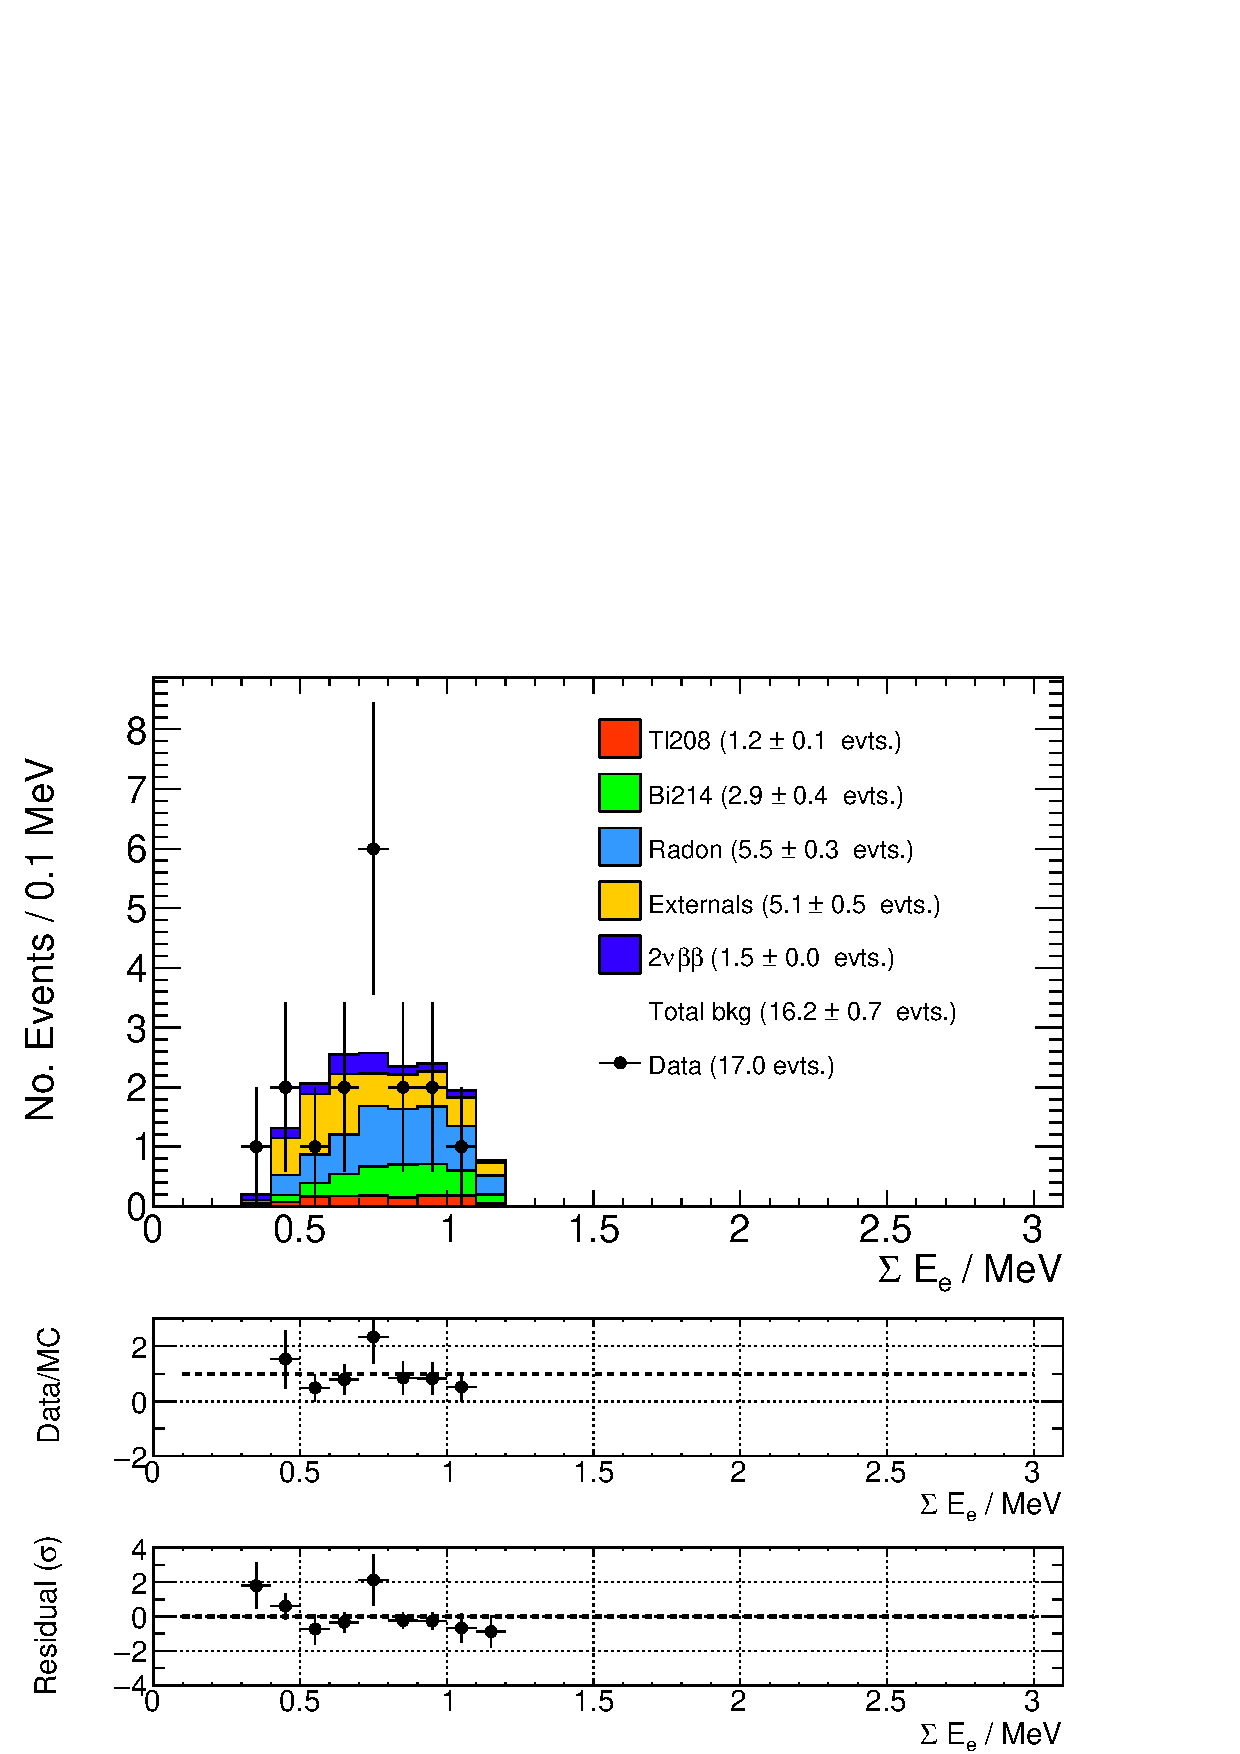
\includegraphics[scale=0.5]{pictures/FinalResults/bb2nu2/150/SEe_bb2nu2NS.pdf}
\includegraphics[scale=0.5]{pictures/FinalResults/bb2nu2/150/Eg_bb2nu2NS.pdf}
\end{center}
\caption{Top : Total electron energy in the 2e1$\gamma$ channel. Bottom : Photon energy in the 2e1$\gamma$ channel. The mininal energy of each electron is 150~keV.}
\label{plot:SEeAndEg250bb2nu2_150}
\end{figure}



\begin{figure} [h!]
\begin{center}
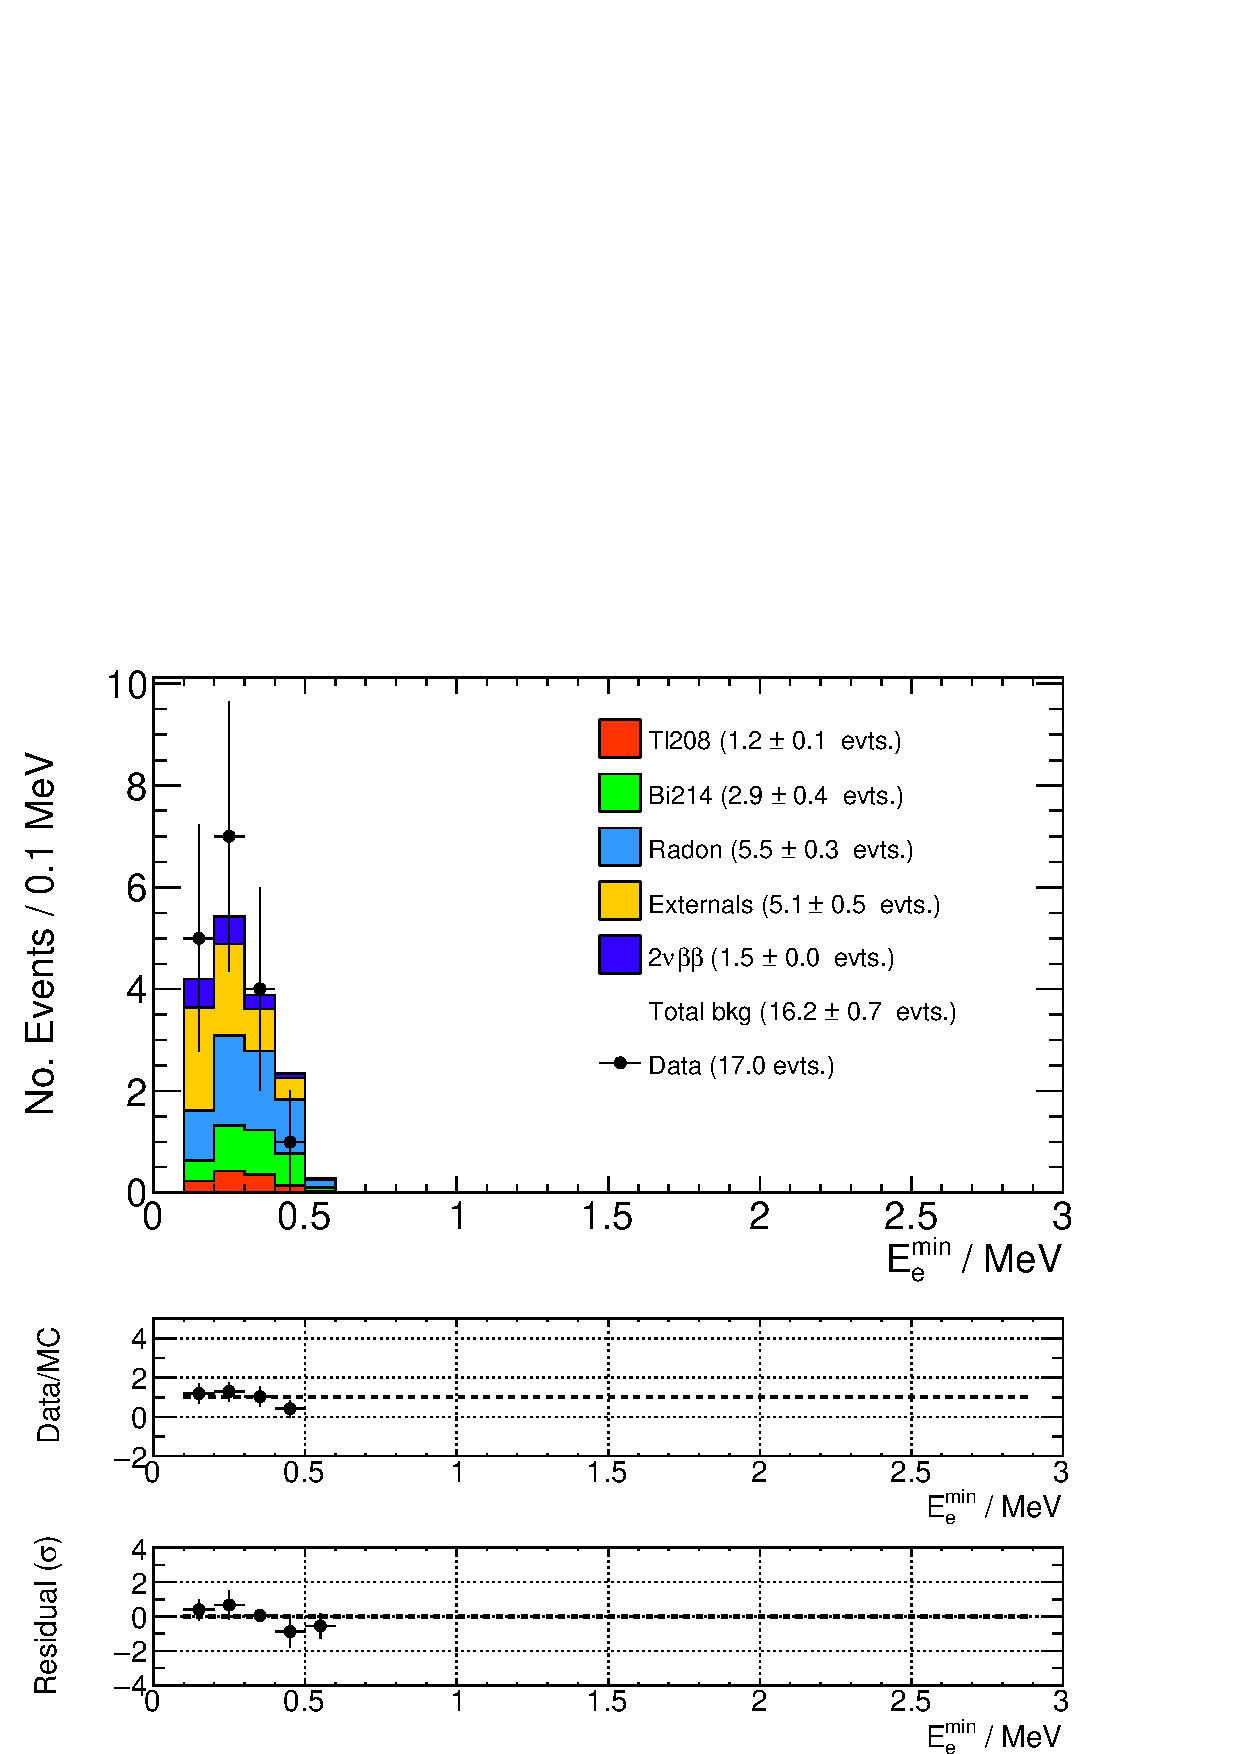
\includegraphics[scale=0.5]{pictures/FinalResults/bb2nu2/150/Eemin_bb2nu2NS.pdf}
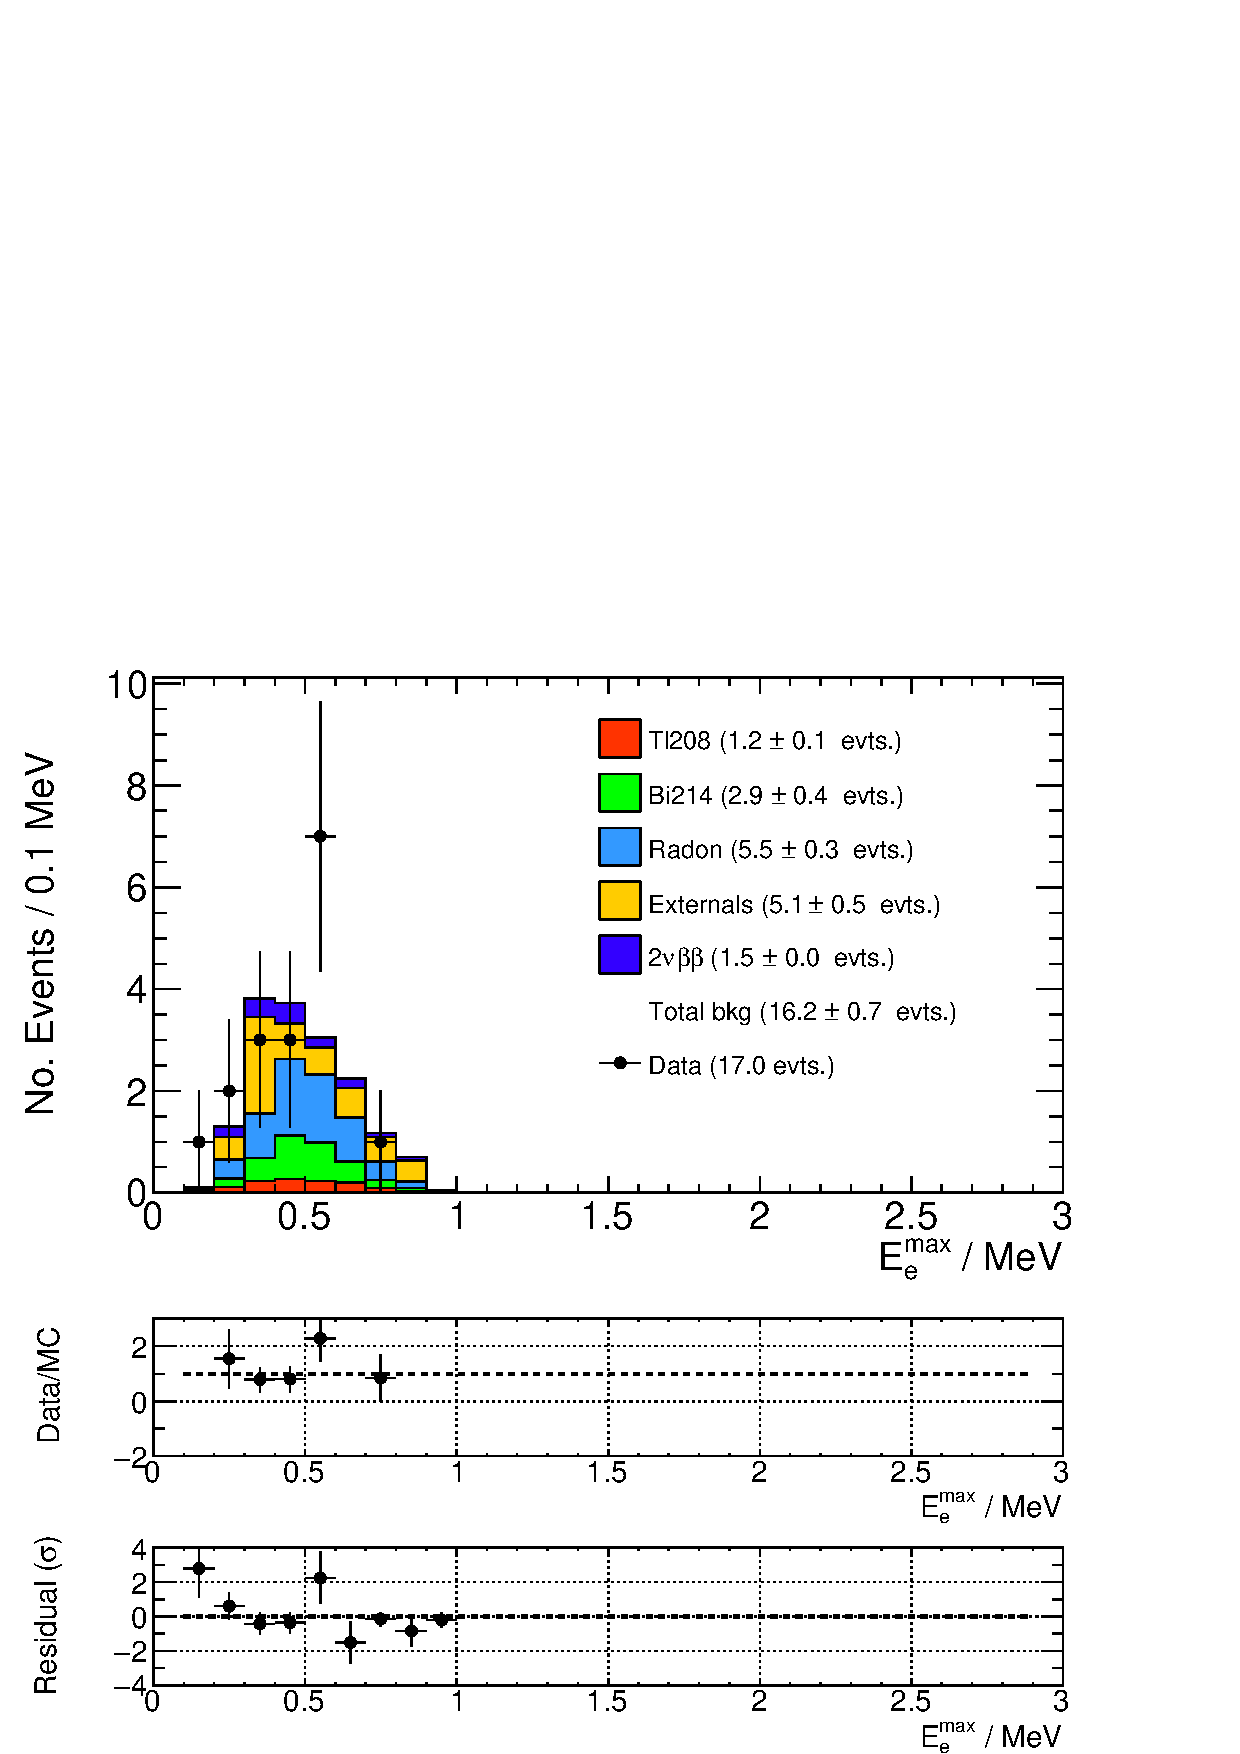
\includegraphics[scale=0.5]{pictures/FinalResults/bb2nu2/150/Eemax_bb2nu2NS.pdf}
\end{center}
\caption{Top : Minimal electron energy in the 2e1$\gamma$ channel. Bottom : Maximal electron energy in the 2e1$\gamma$ channel. The mininal energy of each electron is 150~keV.}
\label{plot:EeminAndEemax250bb2nu2_150}
\end{figure}


\FloatBarrier


\NI From these distributions, it can be seen a small excess of events in the region [0.5~-~0.6]~MeV for the maximal energy of the electron. This small excess corresponds to the small excess of events observed in the sum of energy of the two electrons (between [0.7~-~0.8]~MeV). On the 7 events observed in the bin 0.5~-~0.6~MeV for the maximal energy of the electron, 4 of them have a very small minimal electron energy lower than 250~keV. As no peaked signal is expected in this bin, this small excess could come from an unknown composent of background at low energy which is not taken into account in our background model valid for electron energy greater than 300~keV. 


\bigskip


\NI In order to eliminate this possible source of background, the cut on the minimal energy of each electron is increased to 250~keV and the analysis chain is re-performed. The sensitivity versus the signal efficiency is show in Figure~\ref{plot:SensVsEff_250}. A plateau is observed for signal efficiency between 40\% and 70\% and its the middle value, at 55\%, is chosen. At this signal efficiency 93\% of the background is rejected. The cuts corresponding to select 55\% of the signal are given in Table~\ref{tab:Cuts2nu2Plus250keV}.


\begin{figure} [h!]
\begin{center}
\includegraphics[scale=0.5]{pictures/FinalResults/bb2nu2/250/SensVsEff2nu.pdf}
\end{center}
\caption{Expected sensitivity computed for different value of signal efficiency for the exctited state (2$^+$) 2$\nu$. The black point corresponds to the central value.}
\label{plot:SensVsEff_250}
\end{figure}


\bigskip


\NI By looking at Figure~\ref{Variables14TMVA2nu2}, the cuts can be easily understood. The more relevant cut concerns the photon energy. This cut allows to select the monoenergetic photon emitted in the decay to the excited state by rejecting the low energy photon coming from Bremsstrahlung and high energy photon from $^{\text{208}}$Tl isotope. The cut on the sum energy of the two electrons rejects the events with a high energy. Less contraining cuts on the internal and external probabilities are introduced to reject a part of the external backgrounds. Finally, to reduce the background coming from $\beta\beta$ decay to the ground state, an slight cut on the angle between the electron and the photon is introduced since the photon is expected to be emitted in the same direction as the electron. By taking account these cuts and the efficiency of the preselection, the total signal efficiency, $\epsilon_{\text{tot}}$, is (3.85 $\pm$ 0.06) $\times$ 10$^{-\text{4}}$. 


\FloatBarrier


\begin{table}[h!]
\centering
\begin{tabular}{c|c}
Variables & Selected value \\
\toprule
$\Sigma$E$_{\text{e}}$ & [0.49 - 1.12] \\
E$_{\gamma}$    & [0.45 - 1.41] \\
P$_{\text{int}}^{\text{max}}$ (e-$\gamma$) & [0.024 - 1.000] \\
P$_{\text{ext}}^{\text{min}}$ (e $\rightarrow \gamma$) & [0.00 - 0.44] \\
P$_{\text{ext}}^{\text{min}}$ ($\gamma \rightarrow$ e) & [0.00 - 0.29] \\
cos ($\theta_{\text{e1}-\gamma}$) & [-1.00 - 0.88] \\
cos ($\theta_{\text{e2}-\gamma}$) & [-0.96 - 0.91] \\
\bottomrule
\end{tabular}
\caption{Cuts applied on the preselection to optimise the sensitivity on the half-life of the excited state (2$^+$) 2$\nu$. This selection keeps 55\% of the signal and reject 96\% of the background.}
\label{tab:Cuts2nu2Plus250keV}
\end{table}


\begin{figure} [h!]
\begin{center}
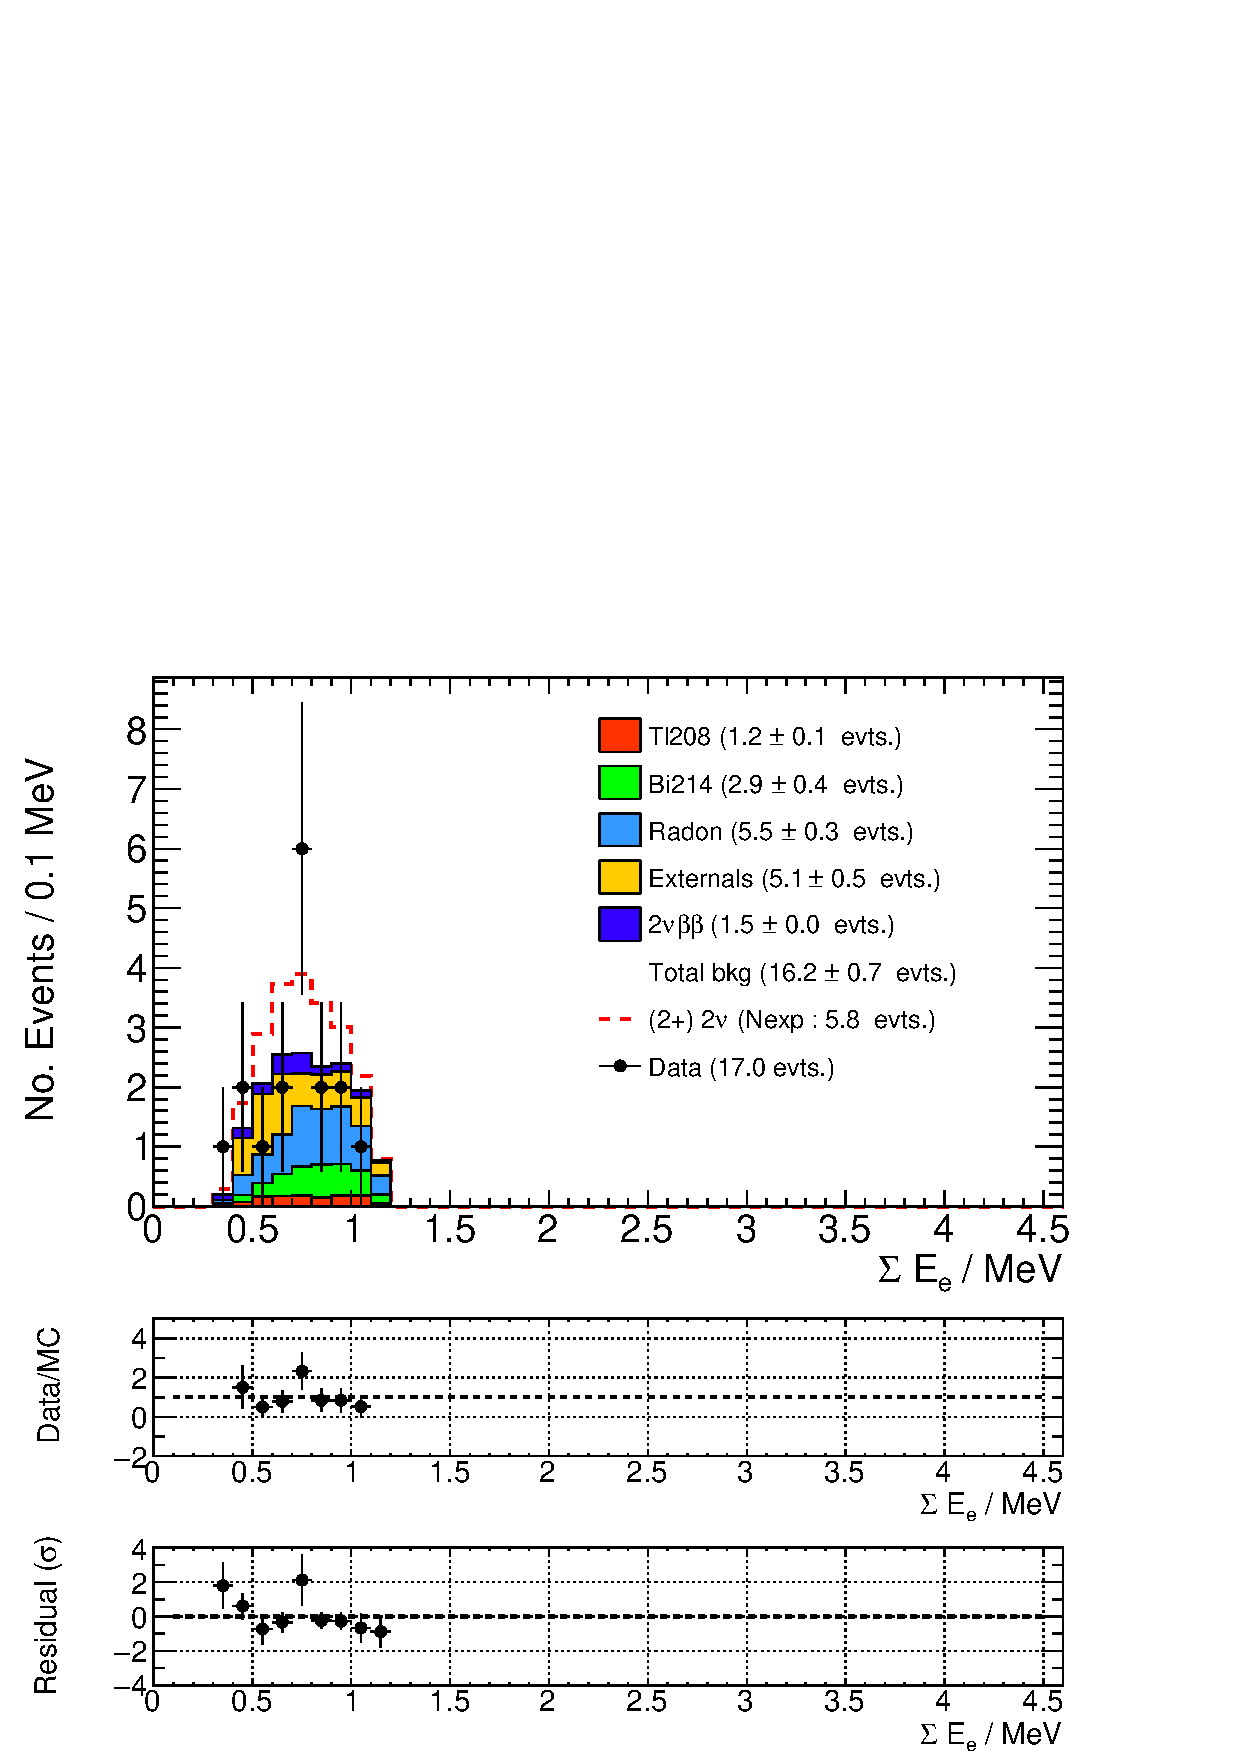
\includegraphics[scale=0.5]{pictures/FinalResults/bb2nu2/250/SEe_bb2nu2.pdf}
\includegraphics[scale=0.5]{pictures/FinalResults/bb2nu2/250/Eg_bb2nu2.pdf}
\end{center}
\caption{Distributions with observed limit in the 2e1$\gamma$ channel for the excited state (2$^+$) 2$\nu$. Top : Total electron energy distribution. Bottom : Photon energy. The mininal energy of each electron is 250~keV.}
\label{plot:SEeAndEg250bb2nu2}
\end{figure}


\begin{figure} [h!]
\begin{center}
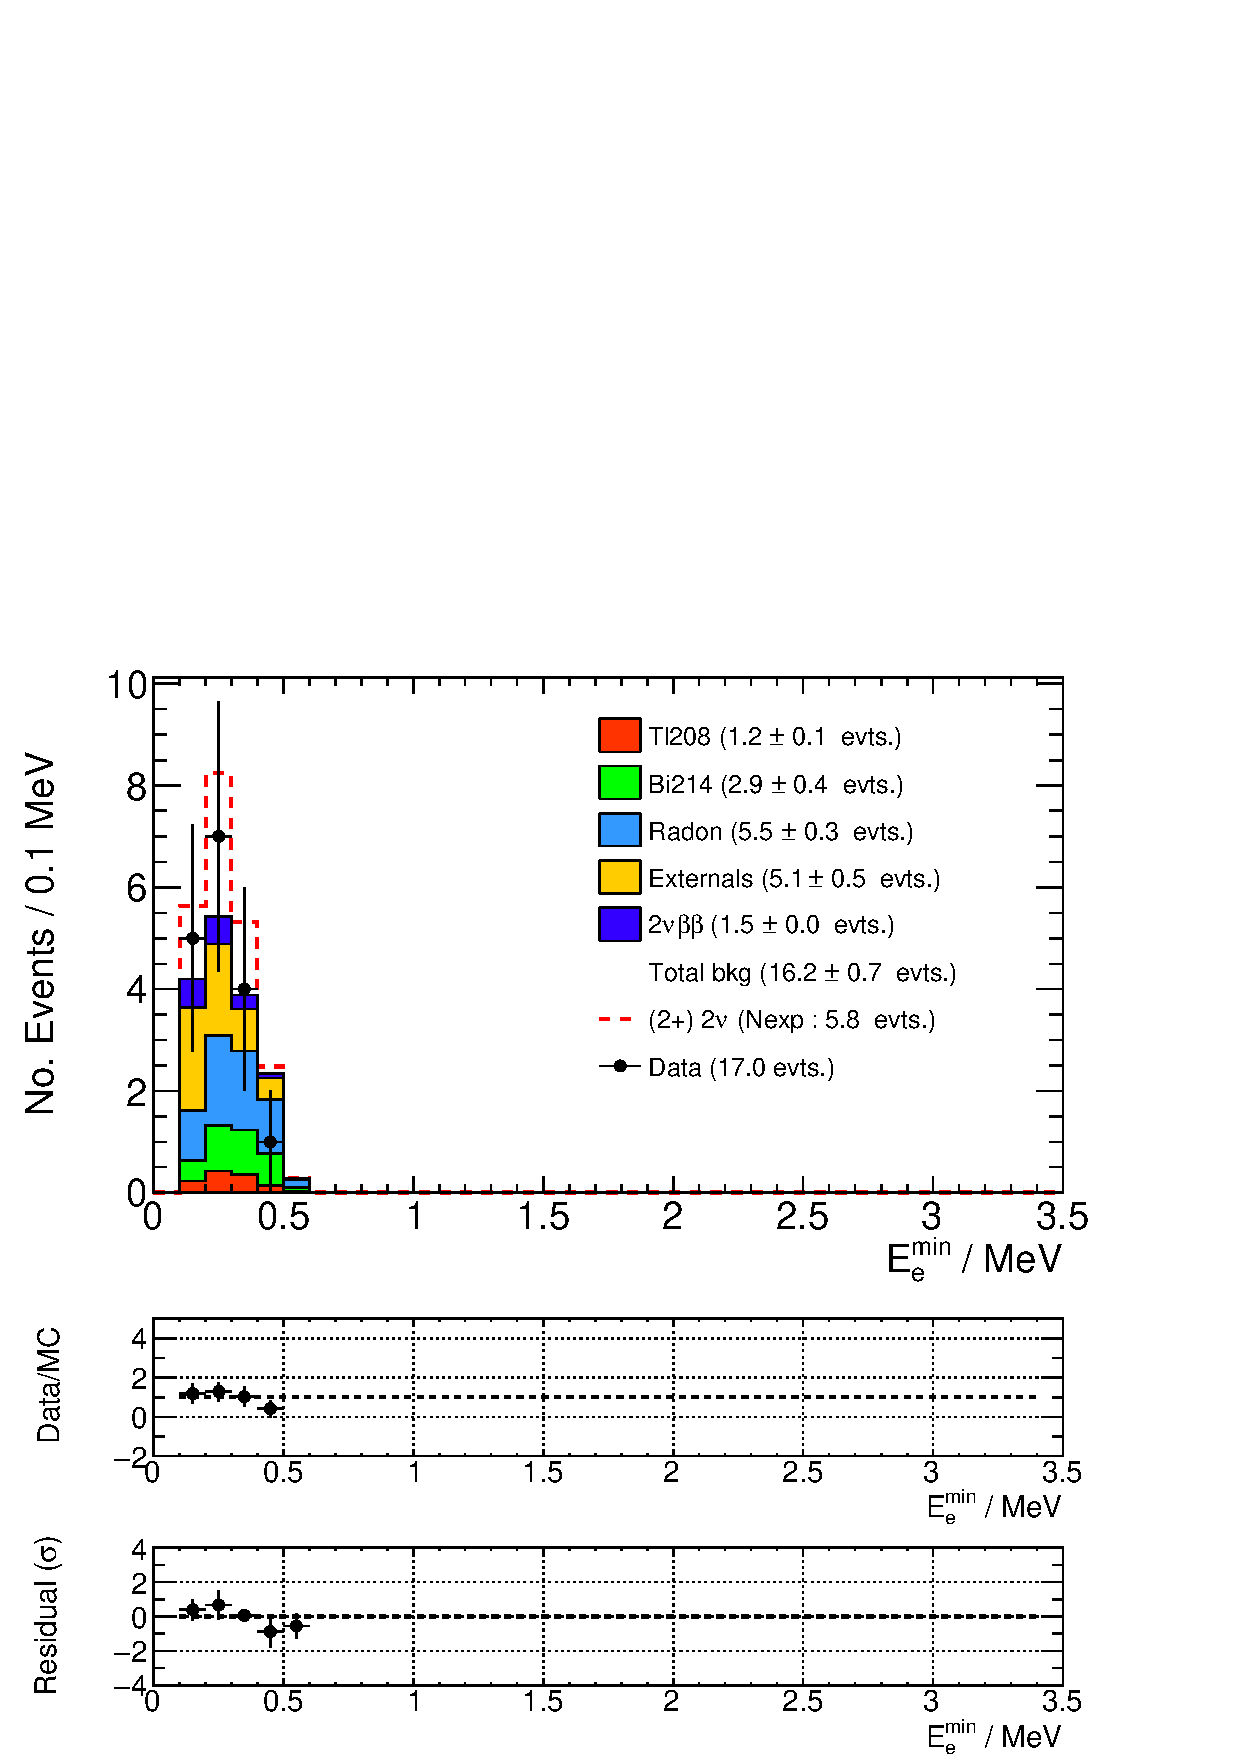
\includegraphics[scale=0.5]{pictures/FinalResults/bb2nu2/250/Eemin_bb2nu2.pdf}
\includegraphics[scale=0.5]{pictures/FinalResults/bb2nu2/250/Eemax_bb2nu2.pdf}
\end{center}
\caption{Distributions with observed limit in the 2e1$\gamma$ channel for the excited state (2$^+$) 2$\nu$. The mininal energy of each electron is 250~keV. Top : Minimal electron energy. Bottom : Maximal electron energy. The mininal energy of each electron is 250~keV.}
\label{plot:EeminAndEemax250bb2nu2}
\end{figure}


\NI As no evidence of signal is observed, an exclusion limit on the signal normalisation is set at 90\% C.L. Table~\ref{Tab:FinalResultsbb2nu2} summarises the expected sensitivity and the observed limit on the signal normalisation as well as the half-life computed from Equation~\ref{sec:SensitivityFormula} and where $\text{N}_{\text{exc.}}^{\text{exp.}}$ is replaced by $\text{N}_{\text{exc.}}^{\text{obs.}}$ for the observed data. The different distributions are shown in Figure~\ref{plot:SEeAndEg250bb2nu2}~and~\ref{plot:EeminAndEemax250bb2nu2}. The observed limit is found to be :



\begin{center}
$ \text{T}_{\text{1/2}}^{\text{2}\nu} (^{\text{116}} \text{Cd}, \text{0} \rightarrow \text{2}^{+}) > \text{4.2} \times \text{10}^{\text{20}}~\text{y}$ at 90\% C.L.
\end{center}


\begin{table}
\centering
\begin{tabular}{c|c|c|c||c}
                                                & -1$\sigma$ & 0        & +1$\sigma$ & obs.     \\[0.2cm]
\hline
%N collie                                       & 9369.6     & 13 520.1 & 19 837.4   & 18 476.6 \\[0.2cm]
N exc.                                          & 3.6        & 5.2      & 7.6        & 7.1      \\[0.2cm]
T$_{\text{1/2}} \times \text{10}^{\text{20}}$y  & 8.28       & 5.74     & 3.91       & 4.2      \\[0.2cm]
\hline
\end{tabular}
\caption{Expected and observed exclusion limit on the signal normalisation and on the half-life at 90\% C.L for the excited state (2$^+$) 2$\nu$.}
\label{Tab:FinalResultsbb2nu2}
\end{table}


\FloatBarrier


\subsection{0$\nu$ decay mode}\label{sec:AnalysisResult2PLUS0nu}


\NI As it has been done for the 2$\nu$ decay mode, the 0$\nu$ analysis is performed in several steps. In a first time, rectangular cuts method is applied on the preselection to find the best cuts at each efficiency. Then the sensitivity is computed for each signal efficiency. The value of the efficiency which maximise the sensitivity is kept as their associated cuts. The final distributions comparing the data to the expected background are shown in Figure~\ref{plot:SEeAndEg250bb0nu2} and \ref{plot:EeminAndEemax250bb0nu2}.



\begin{figure} [h!]
\begin{center}
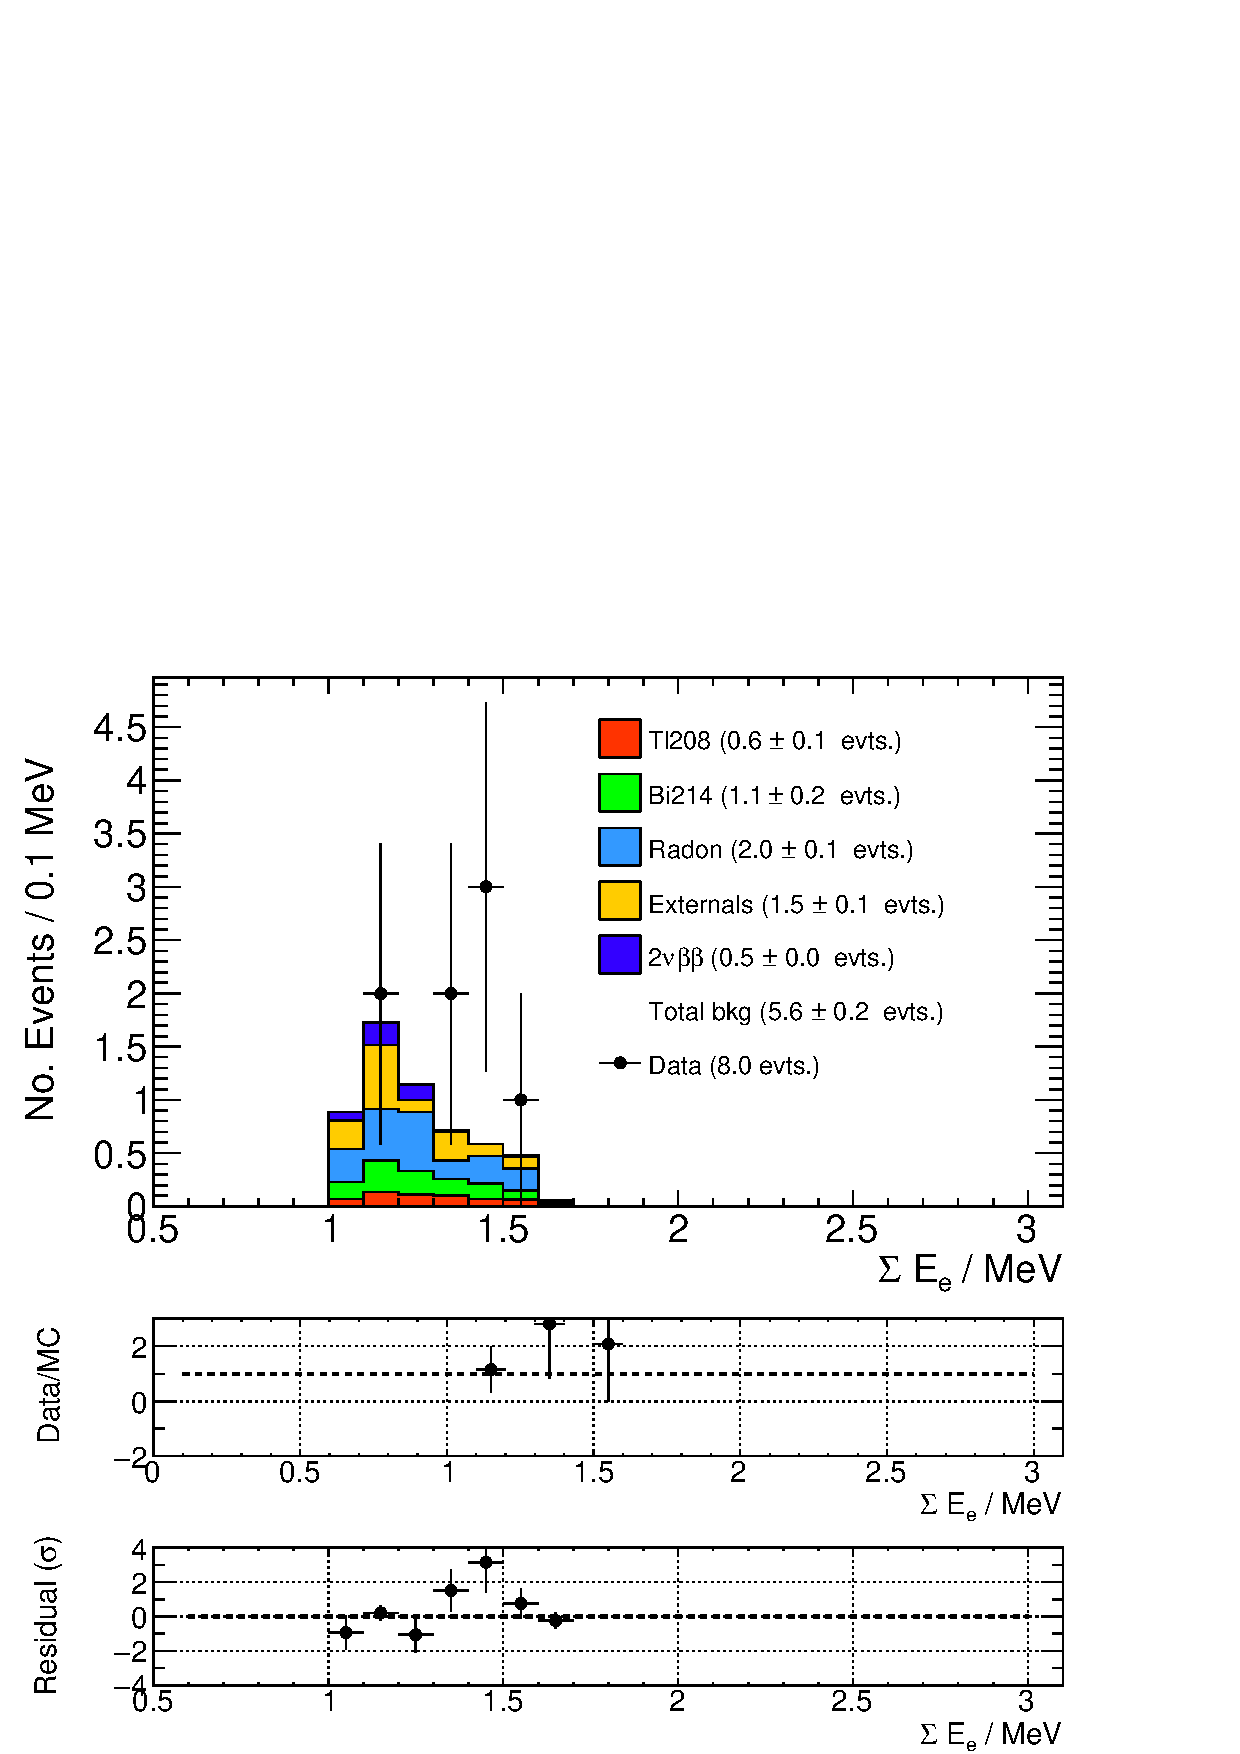
\includegraphics[scale=0.36]{pictures/FinalResults/bb0nu2/150/SEe_bb0nu2NS.pdf}
\includegraphics[scale=0.36]{pictures/FinalResults/bb0nu2/150/Eg_bb0nu2NS.pdf}
\end{center}
\caption{Top : Total electron energy in the 2e1$\gamma$ channel. Bottom : Photon energy in the 2e1$\gamma$ channel. The mininal energy of each electron is 150~keV.}
\label{plot:SEeAndEg250bb0nu2}
\end{figure}


\begin{figure} [h!]
\begin{center}
\includegraphics[scale=0.35]{pictures/FinalResults/bb0nu2/150/Eemin_bb0nu2NS.pdf}
\includegraphics[scale=0.35]{pictures/FinalResults/bb0nu2/150/Eemax_bb0nu2NS.pdf}
\end{center}
\caption{Top : Minimal electron energy in the 2e1$\gamma$ channel. Bottom : Maximal electron energy in the 2e1$\gamma$ channel. The mininal energy of each electron is 150~keV.}
\label{plot:EeminAndEemax250bb0nu2}
\end{figure}


\NI By looking at the photon energy spectrum, 2 events are in excess. The first event have a high energy photon greater than 1.5~MeV and could be interpretated as event coming from $^{\text{208}}$Tl contribution. The second one has internal and external probability which are characteristic of an external event. In order to remove these two events, cut on the maximal energy photon (< 1.6~MeV) and on the probabilities are introduced (P$_\text{int}$ > 0.1 and P$_\text{ext}$ < 0.1) and the cut optimisation is performed again.


\FloatBarrier


\bigskip


\NI The sensitivity versus the signal efficiency is show in Figure~\ref{plot:SensVsEffbb0nu2_250}. A plateau is found between 40\% and 80\%, the middle value is chosen 60\% which corresponds to a total efficiency of (9.34 $\pm$ 0.04 )$\times$ 10$^{-\text{3}}$ and to background rejection of 96\%. The value of the cuts used for this selection is presented in Table~\ref{tab:Cuts0nu2Plus250keV}. The values in red show the cuts introduced before. Note that the external probability values are not in red as these variables have been better constrained during the optimisation process.


\begin{figure} [h!]
\begin{center}
\includegraphics[scale=0.5]{pictures/FinalResults/bb0nu2/SensVsEffbb0nu2.pdf}
\end{center}
\caption{Expected sensitivity computed for different value of signal efficiency for the exctited state (2$^+$) 0$\nu$. The black point corresponds to the central value.}
\label{plot:SensVsEffbb0nu2_250}
\end{figure}


\NI As in 2$\nu$ decay mode, the cut on the photon energy is relevant to select the monoenergetic photon emitted during the decay. The cut on the electron energy is also very important in the 0$\nu$ decay mode since the energy sum of the two electrons is expected to be peaked at the Q$_{\beta\beta}$ value. It explains why the value of this cut is higher in 0$\nu$ case than it is in the 2$\nu$ case. Additionnal slight cuts on the different probabilities are also introduced as well as on the angles. 



\FloatBarrier


\begin{table}[h!]
\centering
\begin{tabular}{c|c}
Variables & Selected value \\
\toprule
$\Sigma$E$_{\text{e}}$ & [0.99 - 1.55] MeV \\
E$_{\gamma}$    & [0.59 - \textcolor{red}{1.6}] MeV \\
P$_{\text{int}}^{\text{max}}$ (e-$\gamma$) & [\textcolor{red}{0.01} - 1.00] \\
P$_{\text{ext}}^{\text{min}}$ (e $\rightarrow \gamma$) & [0.000 - 0.009] \\
P$_{\text{ext}}^{\text{min}}$ ($\gamma \rightarrow$ e) & [0.000 - 0.007] \\
cos ($\theta_{\text{e1}-\gamma}$) & [-1.0 - 0.96] \\
cos ($\theta_{\text{e2}-\gamma}$) & [-1.0 - 0.95] \\
\bottomrule
\end{tabular}
\caption{Cuts applied on the preselection to optimise the sensitivity on the half-life of the excited state (2$^+$) 0$\nu$. This selection keeps 60\% of the signal and reject --\% of the background.}
\label{tab:Cuts0nu2Plus250keV}
\end{table}


%\begin{figure} [h!]
%\begin{center}
%\includegraphics[scale=0.5]{pictures/FinalResults/bb0nu2/150precut/SEe_bb0nu2.pdf}
%\includegraphics[scale=0.5]{pictures/FinalResults/bb0nu2/150precut/Eg_bb0nu2.pdf}
%\end{center}
%\caption{Distributions with observed limit in the 2e1$\gamma$ channel for the excited state (2$^+$) 0$\nu$. Top : Total electron energy distribution. Bottom : Photon energy.}
%\label{plot:SEeAndEg250bb2nu2}\label{plot:SEeAndEg250bb0nu2Precut}
%\end{figure}



\NI  Note that a small excess due to a single event is observed as shown in~Figure~\ref{plot:SEeAndEg250bb0nu2Precut}. The properties of this event are shown in~Table~\ref{tab:EventExcessbb0nu2}. This event could be interpreted as a fluctuation of the external background. If this event is removed the excess disappears.


\begin{table}[h!]
\centering
\begin{tabular}{ccccccc}
\hline
E$^{\text{min}}_\text{e}$ [MeV] & E$^{\text{max}}_\text{e}$ [MeV]& $\Sigma$E$_\text{e}$ [MeV]& E$_{\gamma}$ [MeV]& P$_{\text{int}}^{\text{max}}$ & P$_{\text{ext}}^{\text{min}}$ ($\gamma \rightarrow$ e) & P$_{\text{ext}}^{\text{min}}$ (e $ \rightarrow \gamma$) \\
\hline
0.49 & 0.96 & 1.46 & 0.98 & 0.12 & 0 & 1.4.10$^{-\text{7}}$  \\
\hline
\end{tabular}
\caption{Properties of the event in excess for the decay (2$^+$) 0$\nu$.}
\label{tab:EventExcessbb0nu2}
\end{table}


\bigskip


\NI As no evidence of signal is observed, an exclusion limit on the signal normalisation is set at 90\% C.L. Table~\ref{Tab:FinalResultsbb0nu2} summarises the expected sensitivity and the observed limit on the signal normalisation as well as the half-life. Due to the excess, the limit set on the half-life is below the expected value and is found to be : 


\begin{center}
$ \text{T}_{\text{1/2}}^{\text{0}\nu} (^{\text{116}} \text{Cd}, \text{0} \rightarrow \text{2}^{+}) > \text{7.7} \times \text{10}^{\text{21}}~\text{y}$ at 90\% C.L.
\end{center}


\begin{table}
\centering
\begin{tabular}{c|c|c|c||c}
                                                & -1$\sigma$ & 0        & +1$\sigma$ & obs.     \\[0.2cm]
\hline
%N collie                                       & 292.4      & 394.8    & 586.7      & 1013.2   \\[0.2cm]
N exc.                                          & 2.7        & 3.7      & 5.5        & 9.5      \\[0.2cm]
T$_{\text{1/2}} \times \text{10}^{\text{22}}$y  & 2.65       & 1.97     & 1.32       & 0.77      \\[0.2cm]
\hline
\end{tabular}
\caption{Expected and observed exclusion limit on the signal normalisation and on the half-life at 90\% C.L for the excited state (2$^+$) 0$\nu$.}
\label{Tab:FinalResultsbb0nu2}
\end{table}


\begin{figure} [h!]
\begin{center}
\includegraphics[scale=0.36]{pictures/FinalResults/bb0nu2/150precut/SEe_bb0nu2.pdf}
\includegraphics[scale=0.36]{pictures/FinalResults/bb0nu2/150precut/Eg_bb0nu2.pdf}
\includegraphics[scale=0.36]{pictures/FinalResults/bb0nu2/150precut/Eemin_bb0nu2.pdf}
\includegraphics[scale=0.36]{pictures/FinalResults/bb0nu2/150precut/Eemax_bb0nu2.pdf}
\end{center}
\caption{Distributions with observed limit in the 2e1$\gamma$ channel for the excited state (2$^+$) 0$\nu$. The mininal energy of each electron is 250~keV. Top : Minimal electron energy. Bottom : Maximal electron energy.}
\label{plot:SEeAndEg250bb0nu2Precut}
\end{figure}


\FloatBarrier


\section{$\beta\beta$ decay of $^{\text{116}}$Cd via the excited state (0$^+$) of $^{\text{116}}$Sn}\label{sec:Result0PLUS}


\NI This section presents the results obtained in the search for the double beta decay of \Cd ~ to \Sn ~via the excited state  (0$^+$). The strategy adopted for this investigation is similar to the strategy used for the search for decay via the excited state (2$^+$). The only difference is that the optimisation of the cuts is perfomed on the events of the 2e2$\gamma$ channels. The results of both 2$\nu$ and  0$\nu$ decay modes are respectively presented in Section~\ref{Analysisbb2nu0} and~\ref{Analysisbb0nu0}.


\subsection{2$\nu$ decay mode}\label{Analysisbb2nu0}


\NI After the optimisation of the cuts by TMVA, the sensitivity is maximized for a signal efficiency of 65\%. The corresponding cuts are applied on the preselected events. The final distributions are shown is Figure~\ref{plot:EeminAndEemax250bb2nu0_150} and~\ref{plot:SEeAndEg250bb2nu0_150}. 


\begin{figure} [h!]
\begin{center}
\includegraphics[scale=0.36]{pictures/FinalResults/bb2nu0/150/Eemin_bb2nu0NS.pdf}
\includegraphics[scale=0.36]{pictures/FinalResults/bb2nu0/150/Eemax_bb2nu0NS.pdf}
\end{center}
\caption{Distributions in the 2e2$\gamma$ channel for the excited state (0$^+$) 2$\nu$. The mininal energy of each electron is 150~keV. Top : Minimal electron energy. Bottom : Maximal electron energy.}
\label{plot:EeminAndEemax250bb2nu0_150}
\end{figure}


\begin{figure} [h!]
\begin{center}
\includegraphics[scale=0.36]{pictures/FinalResults/bb2nu0/150/SEe_bb2nu0NS.pdf}
\includegraphics[scale=0.36]{pictures/FinalResults/bb2nu0/150/Eg_bb2nu0NS.pdf}
\includegraphics[scale=0.37]{pictures/FinalResults/bb2nu0/150/EgMin_bb2nu0NS.pdf}
\end{center}
\caption{Distributions in the 2e2$\gamma$ channel for the excited state (0$^+$) 2$\nu$. The mininal energy of each electron is 150~keV. Top : Minimal electron energy. Bottom : Maximal electron energy.}
\label{plot:SEeAndEg250bb2nu0_150}
\end{figure}


\NI From these distributions, an excess of events is observed for all the observables. This excess could come from the same unknown background component discussed in Section~\ref{sec:AnalysisResult2PLUS2nu} since the minimal energy of the electron, for these 6 events, is lower than 250~keV. Futhermore, as the available energy for the electrons is reduced in (0$^+$) excited state, an unknown background composant at low energy could be more troublesome than it was for the excited state (2$^+$). In order to suppress this excess, the cut on the minimal energy of the electron is increased to 250~keV and the optimisation of the cuts by TMVA is performed again.


\bigskip


\NI After the optimisation of the selection, it has been found that the sensitivity is maximized for a signal efficiency of 60\% from the preselection as shown in Figure~\ref{plot:SensVsEffbb2nu0_250}. The cuts corresponding to this selection efficiency are given in Table~\ref{tab:Cuts2nu0Plus250keV}. This selection allow to reject 92\% of the background.


\begin{figure} [h!]
\begin{center}
\includegraphics[scale=0.5]{pictures/FinalResults/bb2nu0/SensVsEff_bb2nu0_250.pdf}
\end{center}
\caption{Expected sensitivity computed for different value of signal efficiency for the exctited state (0$^+$) 2$\nu$. The black point corresponds to the central value.}
\label{plot:SensVsEffbb2nu0_250}
\end{figure}



\begin{table}[h!]
\centering
\begin{tabular}{c|c}
Variables & Selected value \\
\toprule
$\Sigma$E$_{\text{e}}$ & [0.50 - 0.89] \\
E$_{\gamma}^{\text{min}}$    & [0.15 - 0.56] \\
E$_{\gamma}^{\text{max}}$    & [0.15 - 1.35] \\
P$_{\text{int}}^{\text{max}}$ (e-$\gamma$) & [0.13 - 1.00] \\
P$_{\text{ext}}^{\text{min}}$ (e $\rightarrow \gamma$) & [0.00 - 0.80] \\
P$_{\text{ext}}^{\text{min}}$ ($\gamma \rightarrow$ e) & [0.00 - 0.09] \\
cos ($\theta_{\text{e1}-\gamma}$) & [-0.99 - 0.98] \\
cos ($\theta_{\text{e2}-\gamma}$) & [-1.00 - 0.98] \\
\bottomrule
\end{tabular}
\caption{Cuts applied on the preselection to optimise the sensitivity on the half-life of the excited state (0$^+$) 2$\nu$. This selection keeps 60\% of the signal and reject 92\% of the background.}
\label{tab:Cuts2nu0Plus250keV}
\end{table}


\bigskip


\NI The more important cuts concern the energy of the photons. Two monoenergetic photons are emitted at 463~keV and 1294~keV and are kept by the selection. The cut on the electron energy select the signal spectrum with a Q$_{\beta\beta}$ velue at 1048~keV. Additionnal cuts on the probabilities and and angles are introduced to remove external background and events coming from $\beta\beta$ decay to the fundamental state. The final signal efficiency is then (8.98 $\pm$ 0.21) $\times$ 10$^{-\text{6}}$. These cuts are applied on the remaining events of the 2e2$\gamma$ preselection. The final distribution are shown in Figure~\ref{plot:SEeAndEg250bb2nu0_250} and~\ref{plot:EeminAndEemax250bb2nu0_250}. 


\bigskip


\NI No evidence of signal is observed. An exclusion limit on the signal normalisation is set at 90\% C.L. Table~\ref{Tab:FinalResultsbb2nu0} summarises the expected sensitivity and the observed limit on the signal normalisation as well as the half-life. The observed limit is found to be : 


\begin{center}
$ \text{T}_{\text{1/2}}^{\text{2}\nu} (^{\text{116}} \text{Cd}, \text{0} \rightarrow \text{0}^{+}) > \text{2.1} \times \text{10}^{\text{19}}~\text{y}$ at 90\% C.L.
\end{center}


\begin{table}
\centering
\begin{tabular}{c|c|c|c||c}
                                                & -1$\sigma$ & 0        & +1$\sigma$ & obs.     \\[0.2cm]
\hline
N exc.                                          & 2.56       & 3.5      & 5.0          & 3.3     \\[0.2cm]
T$_{\text{1/2}} \times \text{10}^{\text{19}}$y  & 2.7        & 2.0      & 1.4          & 2.1      \\[0.2cm]
\hline 
\end{tabular}
\caption{Expected and observed exclusion limit on the signal normalisation and on the half-life at 90\% C.L for the excited state (0$^+$) 2$\nu$.}
\label{Tab:FinalResultsbb2nu0}
\end{table}


\begin{figure} [h!]
\begin{center}
\includegraphics[scale=0.36]{pictures/FinalResults/bb2nu0/250/Eemin_bb2nu0_60.pdf}
\includegraphics[scale=0.36]{pictures/FinalResults/bb2nu0/250/Eemax_bb2nu0_60.pdf}
\end{center}
\caption{Distributions in the 2e2$\gamma$ channel for the excited state (0$^+$) 2$\nu$. The mininal energy of each electron is 150~keV. Top : Minimal electron energy. Bottom : Maximal electron energy.}
\label{plot:EeminAndEemax250bb2nu0_250}
\end{figure}


\begin{figure} [h!]
\begin{center}
\includegraphics[scale=0.36]{pictures/FinalResults/bb2nu0/250/SEe_bb2nu0_60.pdf}
\includegraphics[scale=0.36]{pictures/FinalResults/bb2nu0/250/Eg_bb2nu0_60.pdf}
\includegraphics[scale=0.36]{pictures/FinalResults/bb2nu0/250/EgMin_bb2nu0_60.pdf}
\end{center}
\caption{Distributions in the 2e2$\gamma$ channel for the excited state (0$^+$) 2$\nu$. The mininal energy of each electron is 150~keV. Top : Minimal electron energy. Bottom : Maximal electron energy.}
\label{plot:SEeAndEg250bb2nu0_250}
\end{figure}


\FloatBarrier


\subsection{0$\nu$ decay mode}\label{Analysisbb0nu0}


\NI The analysis of this excited state is performed exactly in the same way as the other. The optimisation of the cuts is realized with TMVA on the preselection of the 2e2$\gamma$ channel (with the cut on the minimal energy at 150~keV). As before an excess of events is observed. Six on the seven observed events have an electron with an energy lower than 250~keV. This cut is then increased to 250~keV and the optimisation redone.


\bigskip


\NI The sensitivity against the signal efficiency is shown in Figure~\ref{plot:SensVsEffbb0nu0_250}. The value maximising the sensitivity is at 80\% for a total efficiency of (1.96 $\pm$ 0.02) $\times$ 10$^{-\text{3}}$ and corresponds to reject 89\% of the background. The associated cuts are gathered in Table~\ref{tab:Cuts0nu0Plus250keV} and are applied on the events of the 2e2$\gamma$ preselection.


\begin{figure} [h!]
\begin{center}
\includegraphics[scale=0.55]{pictures/FinalResults/bb0nu0/SensVsEff_bb0nu0_250_v2.pdf}
\end{center}
\caption{Expected sensitivity computed for different value of signal efficiency for the exctited state (0$^+$) 0$\nu$. The black point corresponds to the central value.}
\label{plot:SensVsEffbb0nu0_250}
\end{figure}



\begin{table}[h!]
\centering
\begin{tabular}{c|c}
Variables & Selected value \\
\toprule
$\Sigma$E$_{\text{e}}$ & [0.53 - 0.97] \\
E$_{\gamma}^{\text{min}}$    & [0.15 - 0.45] \\
E$_{\gamma}^{\text{max}}$    & [0.15 - 1.34] \\
P$_{\text{int}}^{\text{max}}$ (e-$\gamma$) & [0.1 - 1] \\
P$_{\text{ext}}^{\text{min}}$ (e $\rightarrow \gamma$) & [0.00 - 0.10] \\
P$_{\text{ext}}^{\text{min}}$ ($\gamma \rightarrow$ e) & [0.00 - 0.08] \\
cos ($\theta_{\text{e1}-\gamma}$) & [-1.00 - 0.95] \\
cos ($\theta_{\text{e2}-\gamma}$) & [-0.98 - 1.00] \\
\bottomrule
\end{tabular}
\caption{Cuts applied on the preselection to optimise the sensitivity on the half-life of the excited state (0$^+$) 0$\nu$. This selection keeps 80\% of the signal and reject 88\% of the background.}
\label{tab:Cuts0nu0Plus250keV}
\end{table}


\NI No evidence of signal is observed and an exclusion limit is set at 90\% C.L. The final distributions are shown in Figure~\ref{plot:SEeAndEg250bb0nu0} and~\ref{plot:EeminAndEemax250bb0nu0}. Table~\ref{Tab:FinalResultsbb0nu0} summarises the expected sensitivity and the observed limit on the signal normalisation as well as the half-life. The observed limit is found to be :

\begin{center}
$ \text{T}_{\text{1/2}}^{\text{0}\nu} (^{\text{116}} \text{Cd}, \text{0} \rightarrow \text{0}^{+}) > \text{3.3} \times \text{10}^{\text{21}}~\text{y}$ at 90\% C.L.
\end{center}


\begin{table}
\centering
\begin{tabular}{c|c|c|c||c}
                                                & -1$\sigma$ & 0        & +1$\sigma$ & obs.     \\[0.2cm]
\hline
%N collie                                       & 292.4      & 394.8    & 586.7      & 1013.2   \\[0.2cm]
N exc.                                          & 2.7        & 3.6      & 5.3        & 4.6     \\[0.2cm]
T$_{\text{1/2}} \times \text{10}^{\text{21}}$y  & 5.6        & 4.2      & 2.9        & 3.3      \\[0.2cm]
\hline
\end{tabular}
\caption{Expected and observed exclusion limit on the signal normalisation and on the half-life at 90\% C.L for the excited state (0$^+$) 2$\nu$.}
\label{Tab:FinalResultsbb0nu0}
\end{table}


\begin{figure} [h!]
\begin{center}
\includegraphics[scale=0.36]{pictures/FinalResults/bb0nu0/250/Eemin_bb0nu0_80.pdf}
\includegraphics[scale=0.36]{pictures/FinalResults/bb0nu0/250/Eemax_bb0nu0_80.pdf}
\end{center}
\caption{Distributions with observed limit in the 2e2$\gamma$ channel for the excited state (0$^+$) 0$\nu$. The mininal energy of each electron is 250~keV. Top : Minimal electron energy. Bottom : Maximal electron energy.}
\label{plot:EeminAndEemax250bb0nu0}
\end{figure}


\begin{figure} [h!]
\begin{center}
\includegraphics[scale=0.36]{pictures/FinalResults/bb0nu0/250/SEe_bb0nu0_80.pdf}
\includegraphics[scale=0.36]{pictures/FinalResults/bb0nu0/250/Eg_bb0nu0_80.pdf}
\includegraphics[scale=0.36]{pictures/FinalResults/bb0nu0/250/EgMin_bb0nu0_80.pdf}
\end{center}
\caption{Distributions with observed limit in the 2e2$\gamma$ channel for the excited state (0$^+$) 0$\nu$. The mininal energy of each electron is 250~keV. Top Left : Sum of the electron energy. Top Right : Maximal photon energy. Bottom : Minimal photon energy.}
\label{plot:SEeAndEg250bb0nu0}
\end{figure}


\FloatBarrier


\section{Summary}\label{sec:SummaryAnalysis}


\NI The half-life limits for the $\beta\beta$ decay processes in \Cd ~via the (2$^+$) and (0$^+$) excited state of \Sn ~are summarised in Table~\ref{tab:SummaryResultsAnalysis}. These results are compared with the results obtained by the Aurora experiment~\cite{Aurora} summarised in Table~\ref{tab:AuroraResults}. The Aurora experiment investigates double beta decay of \Cd ~with the help of 1.162~kg cadmium tungstate crystal scintillators enriched in \Cd ~to 82\% which is currently running at LNGS.



\begin{table}[h!]
\centering
\begin{tabular}{c|c|c|c}
Decay mode & $\epsilon$ & N$_{\text{exc.}}^{\text{obs.}}$ & T$_{\text{1/2}}$ at 90\% C.L. \\
\toprule
(2$^+$) 2$\nu$ & 3.84 $\times$ 10$^{-\text{4}}$ & 7.1 & > 4.2 $\times$ 10$^{\text{20}}$ \\[0.2cm]
(2$^+$) 0$\nu$ & 9.34 $\times$ 10$^{-\text{3}}$ & 9.5 & > 7.7 $\times$ 10$^{\text{21}}$ \\[0.2cm]
\hline
(0$^+$) 2$\nu$ & 8.98 $\times$ 10$^{-\text{6}}$ & 3.3 & > 2.1 $\times$ 10$^{\text{19}}$ \\[0.2cm]
(0$^+$) 0$\nu$ & 1.96 $\times$ 10$^{-\text{3}}$ & 4.6 & > 3.3 $\times$ 10$^{\text{21}}$ \\[0.2cm]
\bottomrule
\end{tabular}
\caption{Effciiency, number of excluded event and half-life limits set on the decays of $^{\text{116}}$Cd via the 2 main excited states of $^{\text{116}}$Sn in 2$\nu$ and 0$\nu$ decay modes.}
\label{tab:SummaryResultsAnalysis}
\end{table}


\begin{table}[h!]
\centering
\begin{tabular}{c|c}
Decay mode & T$_{\text{1/2}}$ at 90\% C.L. \\
\toprule
(2$^+$) 2$\nu$ & > 9.0 $\times$ 10$^{\text{20}}$ \\[0.2cm]
(2$^+$) 0$\nu$ & > 6.2 $\times$ 10$^{\text{22}}$ \\[0.2cm]
\hline
(0$^+$) 2$\nu$ & > 1.0 $\times$ 10$^{\text{21}}$ \\[0.2cm]
(0$^+$) 0$\nu$ & > 6.3 $\times$ 10$^{\text{22}}$ \\[0.2cm]
\bottomrule
\end{tabular}
\caption{Half-life limits given at the 90\% C.L. on the $\beta\beta$ decay processes in \Cd ~via the excited state of \Sn. These results have been obtained with CdWO$_\text{4}$ crystal scintillators~\cite{Aurora}.}
\label{tab:AuroraResults}
\end{table}


\NI The results obtained in this work are not competitive with the results from Aurora. This is mainly due to the very low detection efficiency of the NEMO-3 detector compared to the Aurora experiment.


\end{document}
